% Options for packages loaded elsewhere
\PassOptionsToPackage{unicode}{hyperref}
\PassOptionsToPackage{hyphens}{url}
%
\documentclass[
  ignorenonframetext,
]{beamer}
\usepackage{pgfpages}
\setbeamertemplate{caption}[numbered]
\setbeamertemplate{caption label separator}{: }
\setbeamercolor{caption name}{fg=normal text.fg}
\beamertemplatenavigationsymbolsempty
% Prevent slide breaks in the middle of a paragraph
\widowpenalties 1 10000
\raggedbottom
\setbeamertemplate{part page}{
  \centering
  \begin{beamercolorbox}[sep=16pt,center]{part title}
    \usebeamerfont{part title}\insertpart\par
  \end{beamercolorbox}
}
\setbeamertemplate{section page}{
  \centering
  \begin{beamercolorbox}[sep=12pt,center]{part title}
    \usebeamerfont{section title}\insertsection\par
  \end{beamercolorbox}
}
\setbeamertemplate{subsection page}{
  \centering
  \begin{beamercolorbox}[sep=8pt,center]{part title}
    \usebeamerfont{subsection title}\insertsubsection\par
  \end{beamercolorbox}
}
\AtBeginPart{
  \frame{\partpage}
}
\AtBeginSection{
  \ifbibliography
  \else
    \frame{\sectionpage}
  \fi
}
\AtBeginSubsection{
  \frame{\subsectionpage}
}
\usepackage{amsmath,amssymb}
\usepackage{iftex}
\ifPDFTeX
  \usepackage[T1]{fontenc}
  \usepackage[utf8]{inputenc}
  \usepackage{textcomp} % provide euro and other symbols
\else % if luatex or xetex
  \usepackage{unicode-math} % this also loads fontspec
  \defaultfontfeatures{Scale=MatchLowercase}
  \defaultfontfeatures[\rmfamily]{Ligatures=TeX,Scale=1}
\fi
\usepackage{lmodern}
\usetheme[]{Madrid}
\ifPDFTeX\else
  % xetex/luatex font selection
\fi
% Use upquote if available, for straight quotes in verbatim environments
\IfFileExists{upquote.sty}{\usepackage{upquote}}{}
\IfFileExists{microtype.sty}{% use microtype if available
  \usepackage[]{microtype}
  \UseMicrotypeSet[protrusion]{basicmath} % disable protrusion for tt fonts
}{}
\makeatletter
\@ifundefined{KOMAClassName}{% if non-KOMA class
  \IfFileExists{parskip.sty}{%
    \usepackage{parskip}
  }{% else
    \setlength{\parindent}{0pt}
    \setlength{\parskip}{6pt plus 2pt minus 1pt}}
}{% if KOMA class
  \KOMAoptions{parskip=half}}
\makeatother
\usepackage{xcolor}
\newif\ifbibliography
\usepackage{color}
\usepackage{fancyvrb}
\newcommand{\VerbBar}{|}
\newcommand{\VERB}{\Verb[commandchars=\\\{\}]}
\DefineVerbatimEnvironment{Highlighting}{Verbatim}{commandchars=\\\{\}}
% Add ',fontsize=\small' for more characters per line
\usepackage{framed}
\definecolor{shadecolor}{RGB}{248,248,248}
\newenvironment{Shaded}{\begin{snugshade}}{\end{snugshade}}
\newcommand{\AlertTok}[1]{\textcolor[rgb]{0.94,0.16,0.16}{#1}}
\newcommand{\AnnotationTok}[1]{\textcolor[rgb]{0.56,0.35,0.01}{\textbf{\textit{#1}}}}
\newcommand{\AttributeTok}[1]{\textcolor[rgb]{0.13,0.29,0.53}{#1}}
\newcommand{\BaseNTok}[1]{\textcolor[rgb]{0.00,0.00,0.81}{#1}}
\newcommand{\BuiltInTok}[1]{#1}
\newcommand{\CharTok}[1]{\textcolor[rgb]{0.31,0.60,0.02}{#1}}
\newcommand{\CommentTok}[1]{\textcolor[rgb]{0.56,0.35,0.01}{\textit{#1}}}
\newcommand{\CommentVarTok}[1]{\textcolor[rgb]{0.56,0.35,0.01}{\textbf{\textit{#1}}}}
\newcommand{\ConstantTok}[1]{\textcolor[rgb]{0.56,0.35,0.01}{#1}}
\newcommand{\ControlFlowTok}[1]{\textcolor[rgb]{0.13,0.29,0.53}{\textbf{#1}}}
\newcommand{\DataTypeTok}[1]{\textcolor[rgb]{0.13,0.29,0.53}{#1}}
\newcommand{\DecValTok}[1]{\textcolor[rgb]{0.00,0.00,0.81}{#1}}
\newcommand{\DocumentationTok}[1]{\textcolor[rgb]{0.56,0.35,0.01}{\textbf{\textit{#1}}}}
\newcommand{\ErrorTok}[1]{\textcolor[rgb]{0.64,0.00,0.00}{\textbf{#1}}}
\newcommand{\ExtensionTok}[1]{#1}
\newcommand{\FloatTok}[1]{\textcolor[rgb]{0.00,0.00,0.81}{#1}}
\newcommand{\FunctionTok}[1]{\textcolor[rgb]{0.13,0.29,0.53}{\textbf{#1}}}
\newcommand{\ImportTok}[1]{#1}
\newcommand{\InformationTok}[1]{\textcolor[rgb]{0.56,0.35,0.01}{\textbf{\textit{#1}}}}
\newcommand{\KeywordTok}[1]{\textcolor[rgb]{0.13,0.29,0.53}{\textbf{#1}}}
\newcommand{\NormalTok}[1]{#1}
\newcommand{\OperatorTok}[1]{\textcolor[rgb]{0.81,0.36,0.00}{\textbf{#1}}}
\newcommand{\OtherTok}[1]{\textcolor[rgb]{0.56,0.35,0.01}{#1}}
\newcommand{\PreprocessorTok}[1]{\textcolor[rgb]{0.56,0.35,0.01}{\textit{#1}}}
\newcommand{\RegionMarkerTok}[1]{#1}
\newcommand{\SpecialCharTok}[1]{\textcolor[rgb]{0.81,0.36,0.00}{\textbf{#1}}}
\newcommand{\SpecialStringTok}[1]{\textcolor[rgb]{0.31,0.60,0.02}{#1}}
\newcommand{\StringTok}[1]{\textcolor[rgb]{0.31,0.60,0.02}{#1}}
\newcommand{\VariableTok}[1]{\textcolor[rgb]{0.00,0.00,0.00}{#1}}
\newcommand{\VerbatimStringTok}[1]{\textcolor[rgb]{0.31,0.60,0.02}{#1}}
\newcommand{\WarningTok}[1]{\textcolor[rgb]{0.56,0.35,0.01}{\textbf{\textit{#1}}}}
\usepackage{graphicx}
\makeatletter
\def\maxwidth{\ifdim\Gin@nat@width>\linewidth\linewidth\else\Gin@nat@width\fi}
\def\maxheight{\ifdim\Gin@nat@height>\textheight\textheight\else\Gin@nat@height\fi}
\makeatother
% Scale images if necessary, so that they will not overflow the page
% margins by default, and it is still possible to overwrite the defaults
% using explicit options in \includegraphics[width, height, ...]{}
\setkeys{Gin}{width=\maxwidth,height=\maxheight,keepaspectratio}
% Set default figure placement to htbp
\makeatletter
\def\fps@figure{htbp}
\makeatother
\setlength{\emergencystretch}{3em} % prevent overfull lines
\providecommand{\tightlist}{%
  \setlength{\itemsep}{0pt}\setlength{\parskip}{0pt}}
\setcounter{secnumdepth}{-\maxdimen} % remove section numbering
\logo{
\includegraphics[height=1cm,width=3cm]{logo.png}}
\usetheme{Madrid}
\usefonttheme{serif}
\setbeamertemplate{navigation symbols}{}

\usepackage{amsmath}

\usepackage{graphicx}
\setkeys{Gin}{width=0.5\linewidth} 


\usepackage{booktabs}
\usepackage{longtable}
\usepackage{array}
\usepackage{multirow}
\usepackage{wrapfig}
\usepackage{float}
\usepackage{colortbl}
\usepackage{pdflscape}
\usepackage{tabu}
\usepackage{threeparttable}
\usepackage{threeparttablex}
\usepackage[normalem]{ulem}
\usepackage{makecell}
\usepackage{xcolor}
\ifLuaTeX
  \usepackage{selnolig}  % disable illegal ligatures
\fi
\usepackage{bookmark}
\IfFileExists{xurl.sty}{\usepackage{xurl}}{} % add URL line breaks if available
\urlstyle{same}
\hypersetup{
  pdftitle={Lecture 6},
  pdfauthor={Endri Raco},
  hidelinks,
  pdfcreator={LaTeX via pandoc}}

\title{Lecture 6}
\subtitle{Data Visualization with Python : Seaborn}
\author{Endri Raco}
\date{06 March, 2025}

\begin{document}
\frame{\titlepage}

\begin{frame}[allowframebreaks]
  \tableofcontents[hideallsubsections]
\end{frame}
\section{Introduction to Data Visualization with
Seaborn}\label{introduction-to-data-visualization-with-seaborn}

\section{Introduction to Seaborn}\label{introduction-to-seaborn}

\begin{frame}[fragile]{Making a scatter plot with lists}
\phantomsection\label{making-a-scatter-plot-with-lists}
In this exercise, we'll use a dataset that contains information about
227 countries.

\AddToHookNext{env/Highlighting/begin}{\tiny}

\begin{Shaded}
\begin{Highlighting}[]
\ImportTok{import}\NormalTok{ pandas }\ImportTok{as}\NormalTok{ pd}
\ImportTok{import}\NormalTok{ matplotlib.pyplot }\ImportTok{as}\NormalTok{ plt}

\CommentTok{\# URL for the dataset}
\NormalTok{url }\OperatorTok{=} \StringTok{"https://raw.githubusercontent.com/endri81/DataVisualization/refs/heads/main/data/countries{-}of{-}the{-}world.csv"}
\end{Highlighting}
\end{Shaded}
\end{frame}

\begin{frame}[fragile]{Making a scatter plot with lists}
\phantomsection\label{making-a-scatter-plot-with-lists-1}
\AddToHookNext{env/Highlighting/begin}{\tiny}

\begin{Shaded}
\begin{Highlighting}[]
\CommentTok{\# Load the dataset into a DataFrame}
\NormalTok{df }\OperatorTok{=}\NormalTok{ pd.read\_csv(url)}
\CommentTok{\# Process columns by replacing commas with periods and converting to float}
\NormalTok{gdp }\OperatorTok{=} \BuiltInTok{list}\NormalTok{(}\BuiltInTok{map}\NormalTok{(}\BuiltInTok{float}\NormalTok{, [word.replace(}\StringTok{","}\NormalTok{, }\StringTok{"."}\NormalTok{) }\ControlFlowTok{for}\NormalTok{ word }\KeywordTok{in}\NormalTok{ df[}\StringTok{"GDP ($ per capita)"}\NormalTok{].astype(}\BuiltInTok{str}\NormalTok{)]))}
\NormalTok{phones }\OperatorTok{=} \BuiltInTok{list}\NormalTok{(}\BuiltInTok{map}\NormalTok{(}\BuiltInTok{float}\NormalTok{, [word.replace(}\StringTok{","}\NormalTok{, }\StringTok{"."}\NormalTok{) }\ControlFlowTok{for}\NormalTok{ word }\KeywordTok{in}\NormalTok{ df[}\StringTok{"Phones (per 1000)"}\NormalTok{].astype(}\BuiltInTok{str}\NormalTok{)]))}
\NormalTok{percent\_literate }\OperatorTok{=} \BuiltInTok{list}\NormalTok{(}\BuiltInTok{map}\NormalTok{(}\BuiltInTok{float}\NormalTok{, [word.replace(}\StringTok{","}\NormalTok{, }\StringTok{"."}\NormalTok{) }\ControlFlowTok{for}\NormalTok{ word }\KeywordTok{in}\NormalTok{ df[}\StringTok{"Literacy (\%)"}\NormalTok{].astype(}\BuiltInTok{str}\NormalTok{)]))}
\end{Highlighting}
\end{Shaded}
\end{frame}

\begin{frame}{Making a scatter plot with lists}
\phantomsection\label{making-a-scatter-plot-with-lists-2}
This dataset has lots of interesting information on each country, such
as the country's birth rates, death rates, and its gross domestic
product (GDP).

GDP is the value of all the goods and services produced in a year,
expressed as dollars per person.
\end{frame}

\begin{frame}{Making a scatter plot with lists}
\phantomsection\label{making-a-scatter-plot-with-lists-3}
We've created three lists of data from this dataset to get you started.

gdp is a list that contains the value of GDP per country, expressed as
dollars per person.

phones is a list of the number of mobile phones per 1,000 people in that
country.
\end{frame}

\begin{frame}{Making a scatter plot with lists}
\phantomsection\label{making-a-scatter-plot-with-lists-4}
Finally, percent\_literate is a list that contains the percent of each
country's population that can read and write.
\end{frame}

\begin{frame}[fragile]{Making a scatter plot with lists}
\phantomsection\label{making-a-scatter-plot-with-lists-5}
\AddToHookNext{env/Highlighting/begin}{\tiny}

\begin{Shaded}
\begin{Highlighting}[]
\ImportTok{import}\NormalTok{ pandas }\ImportTok{as}\NormalTok{ pd}
\ImportTok{import}\NormalTok{ matplotlib.pyplot }\ImportTok{as}\NormalTok{ plt}
\CommentTok{\# URL for the dataset}
\NormalTok{url }\OperatorTok{=} \StringTok{"https://raw.githubusercontent.com/endri81/DataVisualization/refs/heads/main/data/countries{-}of{-}the{-}world.csv"}
\CommentTok{\# Load the dataset into a DataFrame}
\NormalTok{df }\OperatorTok{=}\NormalTok{ pd.read\_csv(url)}
\CommentTok{\# Process columns by replacing commas with periods and converting to float}
\NormalTok{gdp }\OperatorTok{=} \BuiltInTok{list}\NormalTok{(}\BuiltInTok{map}\NormalTok{(}\BuiltInTok{float}\NormalTok{, [word.replace(}\StringTok{","}\NormalTok{, }\StringTok{"."}\NormalTok{) }\ControlFlowTok{for}\NormalTok{ word }\KeywordTok{in}\NormalTok{ df[}\StringTok{"GDP ($ per capita)"}\NormalTok{].astype(}\BuiltInTok{str}\NormalTok{)]))}
\NormalTok{phones }\OperatorTok{=} \BuiltInTok{list}\NormalTok{(}\BuiltInTok{map}\NormalTok{(}\BuiltInTok{float}\NormalTok{, [word.replace(}\StringTok{","}\NormalTok{, }\StringTok{"."}\NormalTok{) }\ControlFlowTok{for}\NormalTok{ word }\KeywordTok{in}\NormalTok{ df[}\StringTok{"Phones (per 1000)"}\NormalTok{].astype(}\BuiltInTok{str}\NormalTok{)]))}
\NormalTok{percent\_literate }\OperatorTok{=} \BuiltInTok{list}\NormalTok{(}\BuiltInTok{map}\NormalTok{(}\BuiltInTok{float}\NormalTok{, [word.replace(}\StringTok{","}\NormalTok{, }\StringTok{"."}\NormalTok{) }\ControlFlowTok{for}\NormalTok{ word }\KeywordTok{in}\NormalTok{ df[}\StringTok{"Literacy (\%)"}\NormalTok{].astype(}\BuiltInTok{str}\NormalTok{)]))}
\end{Highlighting}
\end{Shaded}
\end{frame}

\begin{frame}[fragile]{Making a scatter plot with lists}
\phantomsection\label{making-a-scatter-plot-with-lists-6}
\AddToHookNext{env/Highlighting/begin}{\tiny}

\begin{Shaded}
\begin{Highlighting}[]
\CommentTok{\# Import Matplotlib and Seaborn}
\ImportTok{import}\NormalTok{ matplotlib.pyplot }\ImportTok{as}\NormalTok{ plt}
\ImportTok{import}\NormalTok{ seaborn }\ImportTok{as}\NormalTok{ sns}
\CommentTok{\# Create scatter plot with GDP on the x{-}axis and number of phones on the y{-}axis}
\NormalTok{sns.scatterplot(x}\OperatorTok{=}\NormalTok{gdp, y}\OperatorTok{=}\NormalTok{phones)}
\CommentTok{\# Show plot}
\NormalTok{plt.show()}
\end{Highlighting}
\end{Shaded}
\end{frame}

\begin{frame}{Making a scatter plot with lists}
\phantomsection\label{making-a-scatter-plot-with-lists-7}
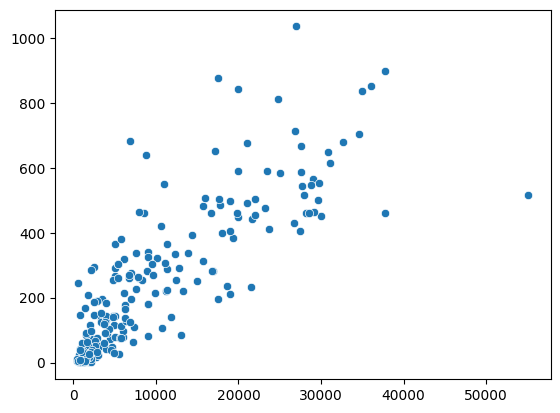
\includegraphics{../images/im253.png}
\end{frame}

\begin{frame}[fragile]{Making a scatter plot with lists}
\phantomsection\label{making-a-scatter-plot-with-lists-8}
\AddToHookNext{env/Highlighting/begin}{\tiny}

\begin{Shaded}
\begin{Highlighting}[]
\CommentTok{\# Change this scatter plot to have percent literate on the y{-}axis}
\NormalTok{sns.scatterplot(x}\OperatorTok{=}\NormalTok{gdp, y}\OperatorTok{=}\NormalTok{percent\_literate)}

\CommentTok{\# Show plot}
\NormalTok{plt.show()}
\end{Highlighting}
\end{Shaded}
\end{frame}

\begin{frame}{Making a scatter plot with lists}
\phantomsection\label{making-a-scatter-plot-with-lists-9}
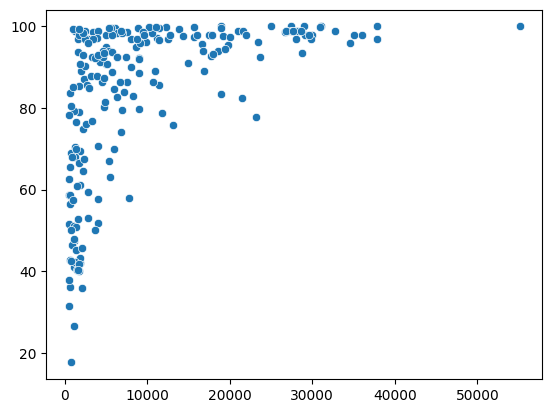
\includegraphics{../images/im254.png}
\end{frame}

\begin{frame}{Making a count plot with a list}
\phantomsection\label{making-a-count-plot-with-a-list}
In the last exercise, we explored a dataset that contains information
about 227 countries.

Let's do more exploration of this data - specifically, how many
countries are in each region of the world?
\end{frame}

\begin{frame}{Making a count plot with a list}
\phantomsection\label{making-a-count-plot-with-a-list-1}
To do this, we'll need to use a count plot.

Count plots take in a categorical list and return bars that represent
the number of list entries per category.
\end{frame}

\begin{frame}{Making a count plot with a list}
\phantomsection\label{making-a-count-plot-with-a-list-2}
You can create one here using a list of regions for each country, which
is a variable named region.
\end{frame}

\begin{frame}[fragile]{Making a count plot with a list}
\phantomsection\label{making-a-count-plot-with-a-list-3}
\AddToHookNext{env/Highlighting/begin}{\tiny}

\begin{Shaded}
\begin{Highlighting}[]
\NormalTok{region }\OperatorTok{=}\NormalTok{ countries[}\StringTok{"Region"}\NormalTok{]}
\CommentTok{\# Import Matplotlib and Seaborn}
\ImportTok{import}\NormalTok{ matplotlib.pyplot }\ImportTok{as}\NormalTok{ plt}
\ImportTok{import}\NormalTok{ seaborn }\ImportTok{as}\NormalTok{ sns}

\CommentTok{\# Create count plot with region on the y{-}axis}
\NormalTok{sns.countplot(y}\OperatorTok{=}\NormalTok{region)}

\CommentTok{\# Show plot}
\NormalTok{plt.show()}
\end{Highlighting}
\end{Shaded}
\end{frame}

\begin{frame}{Making a count plot with a list}
\phantomsection\label{making-a-count-plot-with-a-list-4}
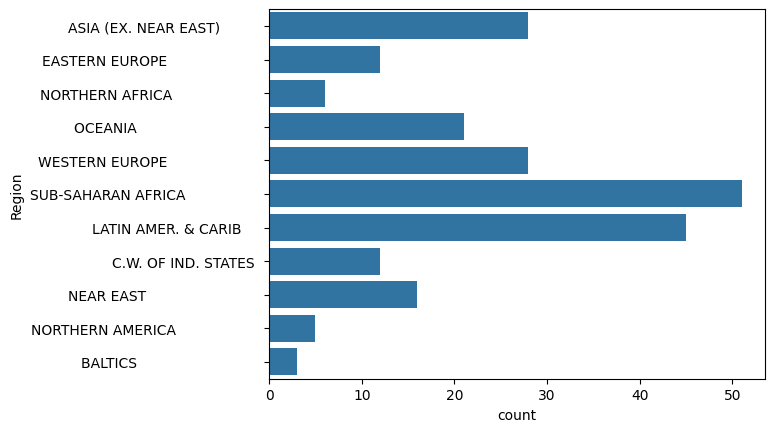
\includegraphics{../images/im255.png}
\end{frame}

\begin{frame}{``Tidy'' vs.~``untidy'' data}
\phantomsection\label{tidy-vs.-untidy-data}
Here, we have a sample dataset from a survey of children about their
favorite animals.

But can we use this dataset as-is with Seaborn? Let's use pandas to
import the csv file with the data collected from the survey and
determine whether it is tidy, which is essential to having it work well
with Seaborn.
\end{frame}

\begin{frame}{``Tidy'' vs.~``untidy'' data}
\phantomsection\label{tidy-vs.-untidy-data-1}
To get you started, the filepath to the csv file has been assigned to
the variable csv\_filepath.

Note that because csv\_filepath is a Python variable, you will not need
to put quotation marks around it when you read the csv.
\end{frame}

\begin{frame}[fragile]{``Tidy'' vs.~``untidy'' data}
\phantomsection\label{tidy-vs.-untidy-data-2}
Read the csv file located at csv\_filepath into a DataFrame named df.

\AddToHookNext{env/Highlighting/begin}{\tiny}

\begin{Shaded}
\begin{Highlighting}[]
\ImportTok{import}\NormalTok{ pandas }\ImportTok{as}\NormalTok{ pd}
\ImportTok{import}\NormalTok{ seaborn }\ImportTok{as}\NormalTok{ sns}
\ImportTok{import}\NormalTok{ matplotlib.pyplot }\ImportTok{as}\NormalTok{ plt}

\CommentTok{\# URL for the dataset}
\NormalTok{url }\OperatorTok{=} \StringTok{"https://raw.githubusercontent.com/endri81/DataVisualization/refs/heads/main/data/example\_csv.csv"}

\CommentTok{\# Load the dataset}
\NormalTok{df }\OperatorTok{=}\NormalTok{ pd.read\_csv(url)}

\CommentTok{\# Rename columns for easier access (handling spaces and special characters)}
\NormalTok{df.columns }\OperatorTok{=}\NormalTok{ [}\StringTok{"Name"}\NormalTok{, }\StringTok{"Age\_or\_Animal"}\NormalTok{]}
\CommentTok{\# Print the head of df}
\BuiltInTok{print}\NormalTok{(df.head())}
\end{Highlighting}
\end{Shaded}

Print the head of df to show the first five rows.
\end{frame}

\begin{frame}{``Tidy'' vs.~``untidy'' data}
\phantomsection\label{tidy-vs.-untidy-data-3}
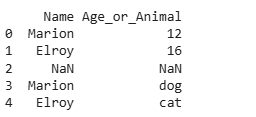
\includegraphics{../images/im256.png}
\end{frame}

\begin{frame}[fragile]{``Tidy'' vs.~``untidy'' data}
\phantomsection\label{tidy-vs.-untidy-data-4}
\AddToHookNext{env/Highlighting/begin}{\tiny}

\begin{Shaded}
\begin{Highlighting}[]
\CommentTok{\# Convert age values to numeric, keeping non{-}numeric (animals) separate}
\NormalTok{df\_numeric }\OperatorTok{=}\NormalTok{ df.copy()}
\NormalTok{df\_numeric[}\StringTok{"Age\_or\_Animal"}\NormalTok{] }\OperatorTok{=}\NormalTok{ pd.to\_numeric(df\_numeric[}\StringTok{"Age\_or\_Animal"}\NormalTok{], errors}\OperatorTok{=}\StringTok{"coerce"}\NormalTok{)}
\end{Highlighting}
\end{Shaded}
\end{frame}

\begin{frame}[fragile]{``Tidy'' vs.~``untidy'' data}
\phantomsection\label{tidy-vs.-untidy-data-5}
\AddToHookNext{env/Highlighting/begin}{\tiny}

\begin{Shaded}
\begin{Highlighting}[]
\CommentTok{\# Plot distribution of numeric values (ages)}
\NormalTok{plt.figure(figsize}\OperatorTok{=}\NormalTok{(}\DecValTok{8}\NormalTok{, }\DecValTok{5}\NormalTok{))}
\NormalTok{sns.histplot(df\_numeric[}\StringTok{"Age\_or\_Animal"}\NormalTok{].dropna(), bins}\OperatorTok{=}\DecValTok{10}\NormalTok{, kde}\OperatorTok{=}\VariableTok{True}\NormalTok{)}
\NormalTok{plt.xlabel(}\StringTok{"Age"}\NormalTok{)}
\NormalTok{plt.ylabel(}\StringTok{"Count"}\NormalTok{)}
\NormalTok{plt.title(}\StringTok{"Distribution of Ages in Dataset"}\NormalTok{)}
\NormalTok{plt.show()}
\end{Highlighting}
\end{Shaded}
\end{frame}

\begin{frame}{``Tidy'' vs.~``untidy'' data}
\phantomsection\label{tidy-vs.-untidy-data-6}
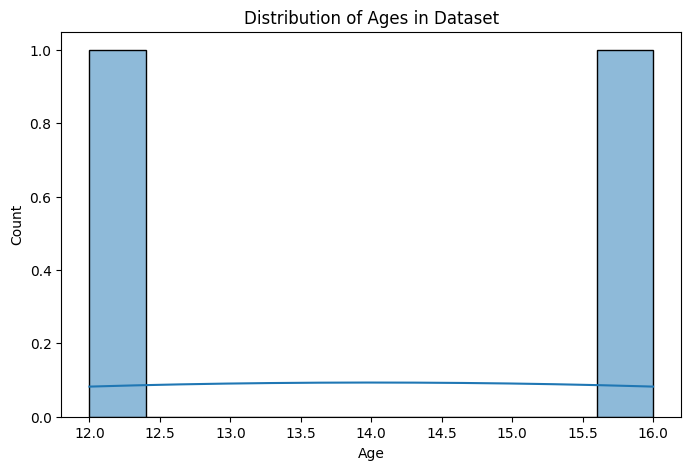
\includegraphics{../images/im257.png}
\end{frame}

\begin{frame}{Making a count plot with a DataFrame}
\phantomsection\label{making-a-count-plot-with-a-dataframe}
In this exercise, we'll look at the responses to a survey sent out to
young people.

Our primary question here is: how many young people surveyed report
being scared of spiders?
\end{frame}

\begin{frame}{Making a count plot with a DataFrame}
\phantomsection\label{making-a-count-plot-with-a-dataframe-1}
Survey participants were asked to agree or disagree with the statement
``I am afraid of spiders''. Responses vary from 1 to 5, where 1 is
``Strongly disagree'' and 5 is ``Strongly agree''.
\end{frame}

\begin{frame}[fragile]{Making a count plot with a DataFrame}
\phantomsection\label{making-a-count-plot-with-a-dataframe-2}
Read the csv file located at csv\_filepath into a DataFrame named df.

\AddToHookNext{env/Highlighting/begin}{\tiny}

\begin{Shaded}
\begin{Highlighting}[]
\ImportTok{import}\NormalTok{ pandas }\ImportTok{as}\NormalTok{ pd}
\ImportTok{import}\NormalTok{ seaborn }\ImportTok{as}\NormalTok{ sns}
\ImportTok{import}\NormalTok{ matplotlib.pyplot }\ImportTok{as}\NormalTok{ plt}

\CommentTok{\# URL for the dataset}
\NormalTok{url }\OperatorTok{=} \StringTok{"https://raw.githubusercontent.com/endri81/DataVisualization/main/data/spiders\_data.csv"}

\CommentTok{\# Load the dataset}
\NormalTok{df }\OperatorTok{=}\NormalTok{ pd.read\_csv(url)}
\end{Highlighting}
\end{Shaded}
\end{frame}

\begin{frame}[fragile]{Making a count plot with a DataFrame}
\phantomsection\label{making-a-count-plot-with-a-dataframe-3}
\AddToHookNext{env/Highlighting/begin}{\tiny}

\begin{Shaded}
\begin{Highlighting}[]
\CommentTok{\# Create a count plot with "Spiders" on the x{-}axis}
\NormalTok{plt.figure(figsize}\OperatorTok{=}\NormalTok{(}\DecValTok{8}\NormalTok{, }\DecValTok{5}\NormalTok{))}
\NormalTok{ax }\OperatorTok{=}\NormalTok{ sns.countplot(x}\OperatorTok{=}\StringTok{"Spiders"}\NormalTok{, data}\OperatorTok{=}\NormalTok{df, palette}\OperatorTok{=}\StringTok{"Set2"}\NormalTok{)}

\CommentTok{\# Annotate bars with values}
\ControlFlowTok{for}\NormalTok{ p }\KeywordTok{in}\NormalTok{ ax.patches:}
\NormalTok{    ax.annotate(}\SpecialStringTok{f\textquotesingle{}}\SpecialCharTok{\{}\NormalTok{p}\SpecialCharTok{.}\NormalTok{get\_height()}\SpecialCharTok{\}}\SpecialStringTok{\textquotesingle{}}\NormalTok{, }
\NormalTok{                (p.get\_x() }\OperatorTok{+}\NormalTok{ p.get\_width() }\OperatorTok{/} \FloatTok{2.}\NormalTok{, p.get\_height()), }
\NormalTok{                ha}\OperatorTok{=}\StringTok{\textquotesingle{}center\textquotesingle{}}\NormalTok{, va}\OperatorTok{=}\StringTok{\textquotesingle{}center\textquotesingle{}}\NormalTok{, fontsize}\OperatorTok{=}\DecValTok{10}\NormalTok{, color}\OperatorTok{=}\StringTok{\textquotesingle{}black\textquotesingle{}}\NormalTok{, }
\NormalTok{                xytext}\OperatorTok{=}\NormalTok{(}\DecValTok{0}\NormalTok{, }\DecValTok{5}\NormalTok{), textcoords}\OperatorTok{=}\StringTok{\textquotesingle{}offset points\textquotesingle{}}\NormalTok{)}
\end{Highlighting}
\end{Shaded}
\end{frame}

\begin{frame}[fragile]{Making a count plot with a DataFrame}
\phantomsection\label{making-a-count-plot-with-a-dataframe-4}
\AddToHookNext{env/Highlighting/begin}{\tiny}

\begin{Shaded}
\begin{Highlighting}[]

\CommentTok{\# Display the plot}
\NormalTok{plt.xlabel(}\StringTok{"Number of Spiders"}\NormalTok{)}
\NormalTok{plt.ylabel(}\StringTok{"Count"}\NormalTok{)}
\NormalTok{plt.title(}\StringTok{"Distribution of Spiders Count"}\NormalTok{)}
\NormalTok{plt.grid(axis}\OperatorTok{=}\StringTok{"y"}\NormalTok{, linestyle}\OperatorTok{=}\StringTok{"{-}{-}"}\NormalTok{, alpha}\OperatorTok{=}\FloatTok{0.7}\NormalTok{)}
\NormalTok{plt.show()}
\end{Highlighting}
\end{Shaded}
\end{frame}

\begin{frame}{Making a count plot with a DataFrame}
\phantomsection\label{making-a-count-plot-with-a-dataframe-5}
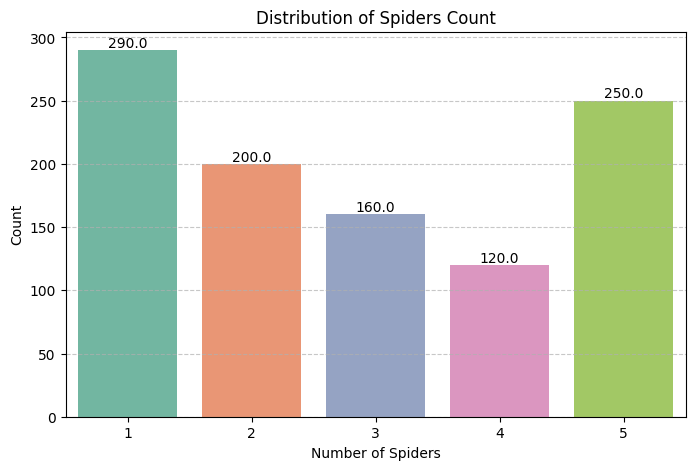
\includegraphics{../images/im258.png}
\end{frame}

\begin{frame}{Hue and scatter plots}
\phantomsection\label{hue-and-scatter-plots}
Previosly, we learned how hue allows us to easily make subgroups within
Seaborn plots.

Let's try it out by exploring data from students in secondary school.

We have a lot of information about each student like their age, where
they live, their study habits and their extracurricular activities.
\end{frame}

\begin{frame}{Hue and scatter plots}
\phantomsection\label{hue-and-scatter-plots-1}
For now, we'll look at the relationship between the number of absences
they have in school and their final grade in the course, segmented by
where the student lives (rural vs.~urban area).
\end{frame}

\begin{frame}[fragile]{Hue and scatter plots}
\phantomsection\label{hue-and-scatter-plots-2}
Create a scatter plot with ``absences'' on the x-axis and final grade
(``G3'') on the y-axis using the DataFrame student\_data.

\AddToHookNext{env/Highlighting/begin}{\tiny}

\begin{Shaded}
\begin{Highlighting}[]
\ImportTok{import}\NormalTok{ pandas }\ImportTok{as}\NormalTok{ pd}
\ImportTok{import}\NormalTok{ seaborn }\ImportTok{as}\NormalTok{ sns}
\ImportTok{import}\NormalTok{ matplotlib.pyplot }\ImportTok{as}\NormalTok{ plt}

\CommentTok{\# URL for the dataset}
\NormalTok{url }\OperatorTok{=} \StringTok{"https://raw.githubusercontent.com/endri81/DataVisualization/refs/heads/main/data/student{-}alcohol{-}consumption.csv"}

\CommentTok{\# Load the dataset}
\NormalTok{df }\OperatorTok{=}\NormalTok{ pd.read\_csv(url)}
\end{Highlighting}
\end{Shaded}
\end{frame}

\begin{frame}[fragile]{Hue and scatter plots}
\phantomsection\label{hue-and-scatter-plots-3}
Color the plot points based on ``location'' (urban vs.~rural).

\AddToHookNext{env/Highlighting/begin}{\tiny}

\begin{Shaded}
\begin{Highlighting}[]
\CommentTok{\# Import Matplotlib and Seaborn}
\ImportTok{import}\NormalTok{ matplotlib.pyplot }\ImportTok{as}\NormalTok{ plt}
\ImportTok{import}\NormalTok{ seaborn }\ImportTok{as}\NormalTok{ sns}
\CommentTok{\# Create a scatter plot of absences vs. final grade}
\NormalTok{sns.scatterplot(x}\OperatorTok{=}\StringTok{"absences"}\NormalTok{, y}\OperatorTok{=}\StringTok{"G3"}\NormalTok{, }
\NormalTok{                data}\OperatorTok{=}\NormalTok{df, }
\NormalTok{                hue}\OperatorTok{=}\StringTok{"location"}\NormalTok{)}
\CommentTok{\# Show plot}
\NormalTok{plt.show()}
\end{Highlighting}
\end{Shaded}
\end{frame}

\begin{frame}[fragile]{Hue and scatter plots}
\phantomsection\label{hue-and-scatter-plots-4}
Make ``Rural'' appear before ``Urban'' in the plot legend.

\AddToHookNext{env/Highlighting/begin}{\tiny}

\begin{Shaded}
\begin{Highlighting}[]
\CommentTok{\# Change the legend order in the scatter plot}
\NormalTok{ sns.scatterplot(x}\OperatorTok{=}\StringTok{"absences"}\NormalTok{, y}\OperatorTok{=}\StringTok{"G3"}\NormalTok{, }
\NormalTok{                data}\OperatorTok{=}\NormalTok{df, }
\NormalTok{                hue}\OperatorTok{=}\StringTok{"location"}\NormalTok{,}
\NormalTok{                hue\_order}\OperatorTok{=}\NormalTok{[}\StringTok{"Rural"}\NormalTok{, }\StringTok{"Urban"}\NormalTok{])}

\CommentTok{\# Show plot}
\NormalTok{plt.show()}
\end{Highlighting}
\end{Shaded}
\end{frame}

\begin{frame}{Hue and scatter plots}
\phantomsection\label{hue-and-scatter-plots-5}
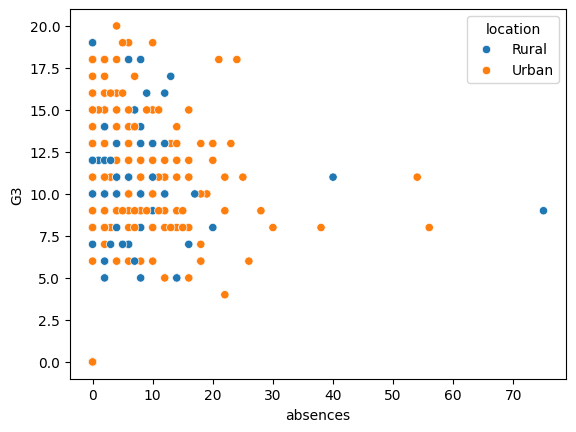
\includegraphics{../images/im260.png}
\end{frame}

\begin{frame}{Hue and count plots}
\phantomsection\label{hue-and-count-plots}
Let's continue exploring our dataset from students in secondary school
by looking at a new variable.

The ``school'' column indicates the initials of which school the student
attended - either ``GP'' or ``MS''.
\end{frame}

\begin{frame}{Hue and count plots}
\phantomsection\label{hue-and-count-plots-1}
In the last exercise, we created a scatter plot where the plot points
were colored based on whether the student lived in an urban or rural
area.

How many students live in urban vs.~rural areas, and does this vary
based on what school the student attends?
\end{frame}

\begin{frame}{Hue and count plots}
\phantomsection\label{hue-and-count-plots-2}
Let's make a count plot with subgroups to find out.
\end{frame}

\begin{frame}[fragile]{Hue and count plots}
\phantomsection\label{hue-and-count-plots-3}
Fill in the palette\_colors dictionary to map the ``Rural'' location
value to the color ``green'' and the ``Urban'' location value to the
color ``blue''.

\AddToHookNext{env/Highlighting/begin}{\tiny}

\begin{Shaded}
\begin{Highlighting}[]
\CommentTok{\# Import Matplotlib and Seaborn}
\ImportTok{import}\NormalTok{ matplotlib.pyplot }\ImportTok{as}\NormalTok{ plt}
\ImportTok{import}\NormalTok{ seaborn }\ImportTok{as}\NormalTok{ sns}

\CommentTok{\# Create a dictionary mapping subgroup values to colors}
\NormalTok{palette\_colors }\OperatorTok{=}\NormalTok{ \{}\StringTok{"Rural"}\NormalTok{: }\StringTok{"green"}\NormalTok{, }\StringTok{"Urban"}\NormalTok{: }\StringTok{"blue"}\NormalTok{\}}
\end{Highlighting}
\end{Shaded}
\end{frame}

\begin{frame}[fragile]{Hue and count plots}
\phantomsection\label{hue-and-count-plots-4}
Create a count plot with ``school'' on the x-axis using the
student\_data DataFrame.

\AddToHookNext{env/Highlighting/begin}{\tiny}

\begin{Shaded}
\begin{Highlighting}[]
\CommentTok{\# Create a count plot of school with location subgroups}
\NormalTok{sns.countplot(x}\OperatorTok{=}\StringTok{"school"}\NormalTok{, data}\OperatorTok{=}\NormalTok{df,}
\NormalTok{              hue}\OperatorTok{=}\StringTok{"location"}\NormalTok{,}
\NormalTok{              palette}\OperatorTok{=}\NormalTok{palette\_colors)}
\end{Highlighting}
\end{Shaded}
\end{frame}

\begin{frame}[fragile]{Hue and count plots}
\phantomsection\label{hue-and-count-plots-5}
Add subgroups to the plot using ``location'' variable and use the
palette\_colors dictionary to make the location subgroups green and
blue.

\AddToHookNext{env/Highlighting/begin}{\tiny}

\begin{Shaded}
\begin{Highlighting}[]
\CommentTok{\# Display plot}
\NormalTok{plt.show()}
\end{Highlighting}
\end{Shaded}
\end{frame}

\begin{frame}{Hue and count plots}
\phantomsection\label{hue-and-count-plots-6}
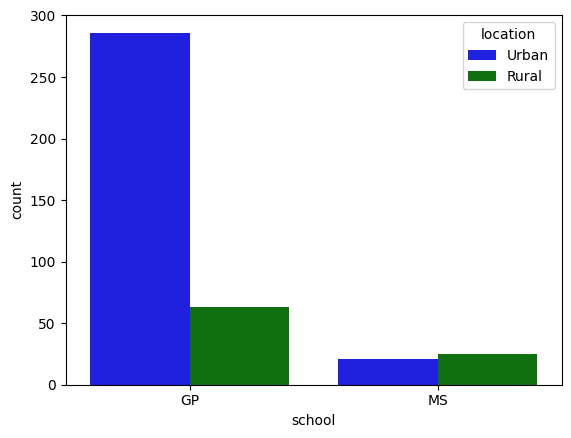
\includegraphics{../images/im261.png}
\end{frame}

\section{Visualizing Two Quantitative
Variables}\label{visualizing-two-quantitative-variables}

\begin{frame}{Creating subplots with col and row}
\phantomsection\label{creating-subplots-with-col-and-row}
We've seen in prior exercises that students with more absences
(``absences'') tend to have lower final grades (``G3'').

Does this relationship hold regardless of how much time students study
each week?
\end{frame}

\begin{frame}{Creating subplots with col and row}
\phantomsection\label{creating-subplots-with-col-and-row-1}
To answer this, we'll look at the relationship between the number of
absences that a student has in school and their final grade in the
course, creating separate subplots based on each student's weekly study
time (``study\_time'').
\end{frame}

\begin{frame}{Creating subplots with col and row}
\phantomsection\label{creating-subplots-with-col-and-row-2}
Seaborn has been imported as sns and matplotlib.pyplot has been imported
as plt.
\end{frame}

\begin{frame}[fragile]{Creating subplots with col and row}
\phantomsection\label{creating-subplots-with-col-and-row-3}
Modify the code to use relplot() instead of scatterplot().

\AddToHookNext{env/Highlighting/begin}{\tiny}

\begin{Shaded}
\begin{Highlighting}[]
\CommentTok{\# Change to use relplot() instead of scatterplot()}
\NormalTok{sns.relplot(x}\OperatorTok{=}\StringTok{"absences"}\NormalTok{, y}\OperatorTok{=}\StringTok{"G3"}\NormalTok{, }
\NormalTok{            data}\OperatorTok{=}\NormalTok{df,}
\NormalTok{            kind}\OperatorTok{=}\StringTok{"scatter"}\NormalTok{)}


\NormalTok{plt.close()}
\end{Highlighting}
\end{Shaded}
\end{frame}

\begin{frame}{Creating subplots with col and row}
\phantomsection\label{creating-subplots-with-col-and-row-4}
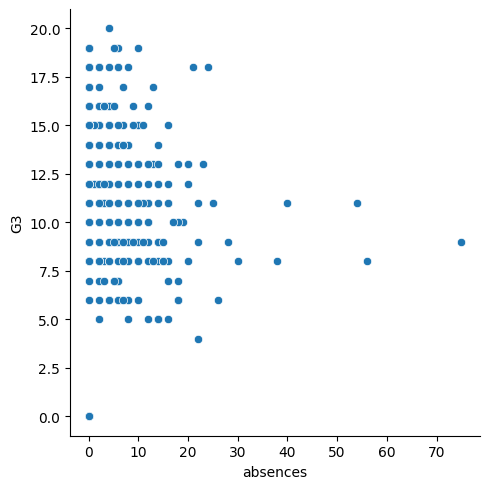
\includegraphics{../images/im262.png}
\end{frame}

\begin{frame}[fragile]{Creating subplots with col and row}
\phantomsection\label{creating-subplots-with-col-and-row-5}
Modify the code to create one scatter plot for each level of the
variable ``study\_time'', arranged in columns.

\AddToHookNext{env/Highlighting/begin}{\tiny}

\begin{Shaded}
\begin{Highlighting}[]
\CommentTok{\# Change to make subplots based on study time}
\NormalTok{sns.relplot(x}\OperatorTok{=}\StringTok{"absences"}\NormalTok{, y}\OperatorTok{=}\StringTok{"G3"}\NormalTok{, }
\NormalTok{            data}\OperatorTok{=}\NormalTok{df,}
\NormalTok{            kind}\OperatorTok{=}\StringTok{"scatter"}\NormalTok{,}
\NormalTok{            col}\OperatorTok{=}\StringTok{"study\_time"}\NormalTok{)}
\NormalTok{plt.show()}
            
\end{Highlighting}
\end{Shaded}
\end{frame}

\begin{frame}{Creating subplots with col and row}
\phantomsection\label{creating-subplots-with-col-and-row-6}
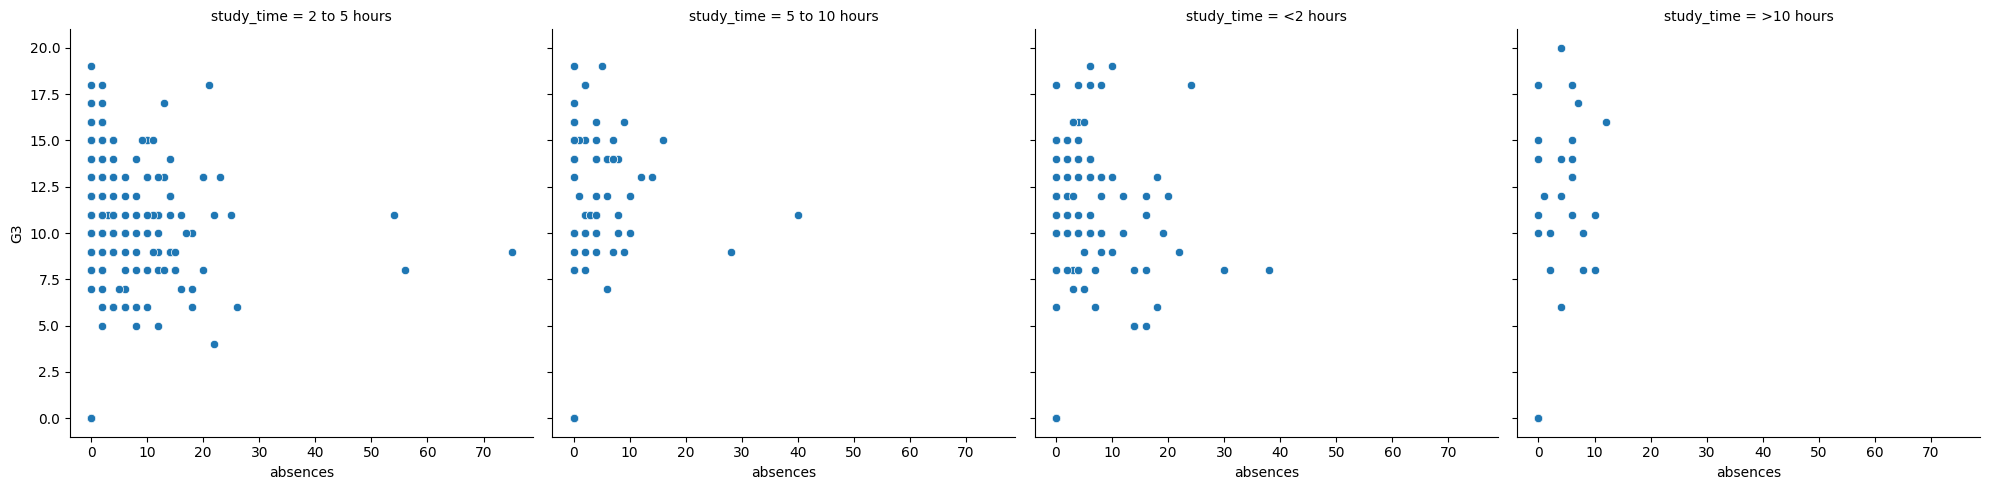
\includegraphics{../images/im263.png}
\end{frame}

\begin{frame}[fragile]{Creating subplots with col and row}
\phantomsection\label{creating-subplots-with-col-and-row-7}
Adapt your code to create one scatter plot for each level of a student's
weekly study time, this time arranged in rows.

\AddToHookNext{env/Highlighting/begin}{\tiny}

\begin{Shaded}
\begin{Highlighting}[]
\CommentTok{\# Change this scatter plot to arrange the plots in rows instead of columns}
\NormalTok{sns.relplot(x}\OperatorTok{=}\StringTok{"absences"}\NormalTok{, y}\OperatorTok{=}\StringTok{"G3"}\NormalTok{, }
\NormalTok{            data}\OperatorTok{=}\NormalTok{student\_data,}
\NormalTok{            kind}\OperatorTok{=}\StringTok{"scatter"}\NormalTok{, }
\NormalTok{            row}\OperatorTok{=}\StringTok{"study\_time"}\NormalTok{)}
\NormalTok{plt.show()}
\end{Highlighting}
\end{Shaded}
\end{frame}

\begin{frame}{Creating subplots with col and row}
\phantomsection\label{creating-subplots-with-col-and-row-8}
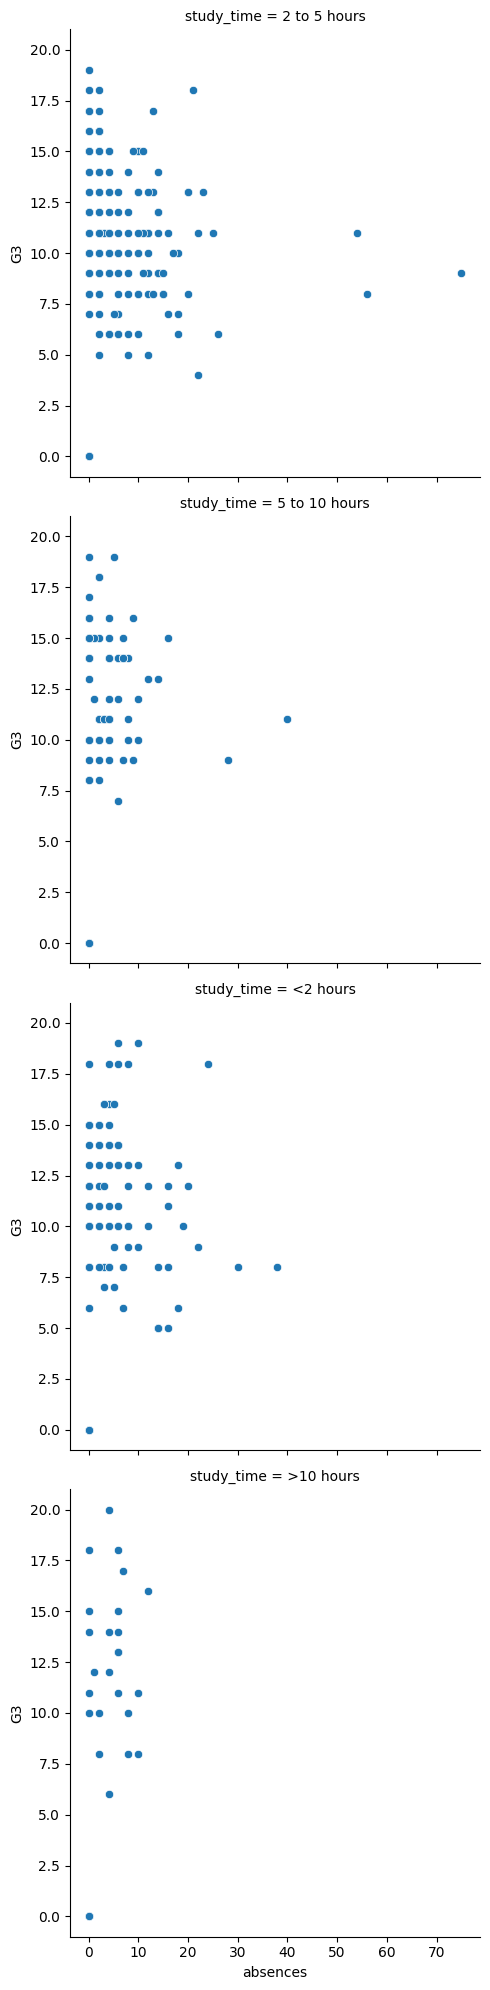
\includegraphics{../images/im264.png}
\end{frame}

\begin{frame}{Creating two-factor subplots}
\phantomsection\label{creating-two-factor-subplots}
Let's continue looking at the student\_data dataset of students in
secondary school.

Here, we want to answer the following question: does a student's first
semester grade (``G1'') tend to correlate with their final grade
(``G3'')?
\end{frame}

\begin{frame}{Creating two-factor subplots}
\phantomsection\label{creating-two-factor-subplots-1}
There are many aspects of a student's life that could result in a higher
or lower final grade in the class.

For example, some students receive extra educational support from their
school (``schoolsup'') or from their family (``famsup''), which could
result in higher grades.
\end{frame}

\begin{frame}{Creating two-factor subplots}
\phantomsection\label{creating-two-factor-subplots-2}
Let's try to control for these two factors by creating subplots based on
whether the student received extra educational support from their school
or family.
\end{frame}

\begin{frame}[fragile]{Creating two-factor subplots}
\phantomsection\label{creating-two-factor-subplots-3}
Use relplot() to create a scatter plot with ``G1'' on the x-axis and
``G3'' on the y-axis, using the student\_data DataFrame.

\AddToHookNext{env/Highlighting/begin}{\tiny}

\begin{Shaded}
\begin{Highlighting}[]
\CommentTok{\# Create a scatter plot of G1 vs. G3}
\NormalTok{sns.relplot(x}\OperatorTok{=}\StringTok{"G1"}\NormalTok{, y}\OperatorTok{=}\StringTok{"G3"}\NormalTok{, }
\NormalTok{            data}\OperatorTok{=}\NormalTok{df,}
\NormalTok{            kind}\OperatorTok{=}\StringTok{"scatter"}\NormalTok{)}
\end{Highlighting}
\end{Shaded}
\end{frame}

\begin{frame}{Creating two-factor subplots}
\phantomsection\label{creating-two-factor-subplots-4}
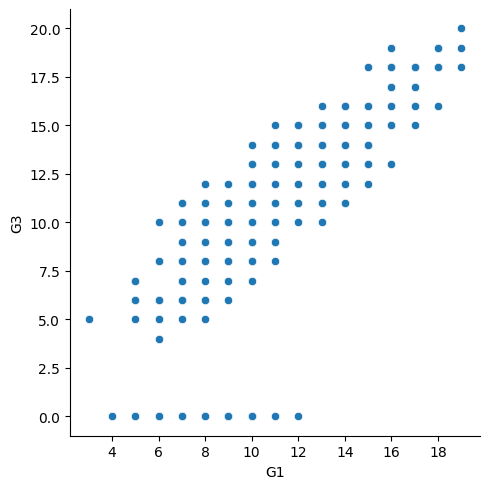
\includegraphics{../images/im265.png}
\end{frame}

\begin{frame}[fragile]{Creating two-factor subplots}
\phantomsection\label{creating-two-factor-subplots-5}
Create column subplots based on whether the student received support
from the school (``schoolsup''), ordered so that ``yes'' comes before
``no''.

\AddToHookNext{env/Highlighting/begin}{\tiny}

\begin{Shaded}
\begin{Highlighting}[]
\CommentTok{\# Adjust to add subplots based on school support}
\NormalTok{sns.relplot(x}\OperatorTok{=}\StringTok{"G1"}\NormalTok{, y}\OperatorTok{=}\StringTok{"G3"}\NormalTok{, }
\NormalTok{            data}\OperatorTok{=}\NormalTok{df,}
\NormalTok{            kind}\OperatorTok{=}\StringTok{"scatter"}\NormalTok{, }
\NormalTok{            col}\OperatorTok{=}\StringTok{"schoolsup"}\NormalTok{,}
\NormalTok{            col\_order}\OperatorTok{=}\NormalTok{[}\StringTok{"yes"}\NormalTok{, }\StringTok{"no"}\NormalTok{])}
\end{Highlighting}
\end{Shaded}
\end{frame}

\begin{frame}{Creating two-factor subplots}
\phantomsection\label{creating-two-factor-subplots-6}
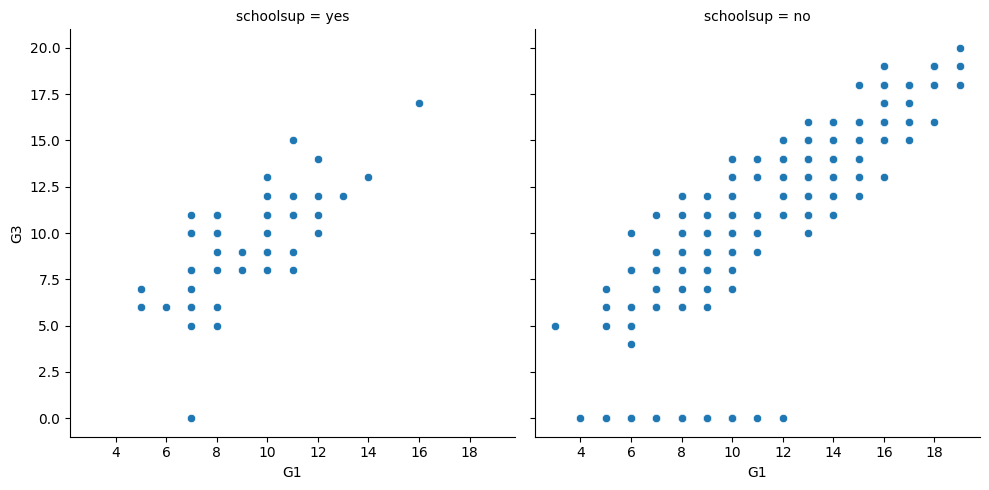
\includegraphics{../images/im266.png}
\end{frame}

\begin{frame}[fragile]{Creating two-factor subplots}
\phantomsection\label{creating-two-factor-subplots-7}
Add row subplots based on whether the student received support from the
family (``famsup''), ordered so that ``yes'' comes before ``no''. This
will result in subplots based on two factors.

\AddToHookNext{env/Highlighting/begin}{\tiny}

\begin{Shaded}
\begin{Highlighting}[]
\CommentTok{\# Adjust further to add subplots based on family support}
\NormalTok{sns.relplot(x}\OperatorTok{=}\StringTok{"G1"}\NormalTok{, y}\OperatorTok{=}\StringTok{"G3"}\NormalTok{, }
\NormalTok{            data}\OperatorTok{=}\NormalTok{df,}
\NormalTok{            kind}\OperatorTok{=}\StringTok{"scatter"}\NormalTok{, }
\NormalTok{            col}\OperatorTok{=}\StringTok{"schoolsup"}\NormalTok{,}
\NormalTok{            col\_order}\OperatorTok{=}\NormalTok{[}\StringTok{"yes"}\NormalTok{, }\StringTok{"no"}\NormalTok{],}
\NormalTok{            row}\OperatorTok{=}\StringTok{"famsup"}\NormalTok{,}
\NormalTok{            row\_order}\OperatorTok{=}\NormalTok{[}\StringTok{"yes"}\NormalTok{, }\StringTok{"no"}\NormalTok{])}
\end{Highlighting}
\end{Shaded}
\end{frame}

\begin{frame}{Creating two-factor subplots}
\phantomsection\label{creating-two-factor-subplots-8}
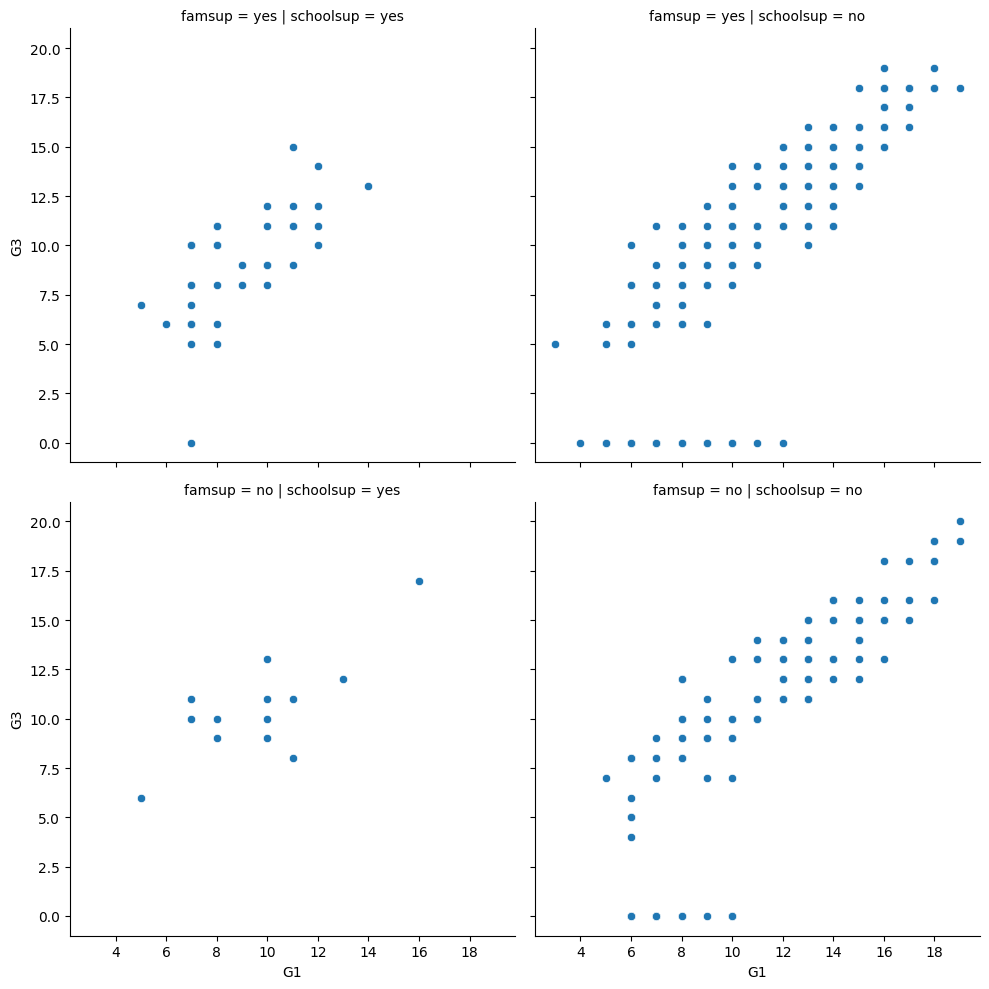
\includegraphics{../images/im267.png}
\end{frame}

\begin{frame}{Changing the size of scatter plot points}
\phantomsection\label{changing-the-size-of-scatter-plot-points}
In this exercise, we'll explore Seaborn's mpg dataset, which contains
one row per car model and includes information such as the year the car
was made, the number of miles per gallon (``M.P.G.'') it achieves, the
power of its engine (measured in ``horsepower''), and its country of
origin.
\end{frame}

\begin{frame}{Changing the size of scatter plot points}
\phantomsection\label{changing-the-size-of-scatter-plot-points-1}
What is the relationship between the power of a car's engine
(``horsepower'') and its fuel efficiency (``mpg'')? And how does this
relationship vary by the number of cylinders (``cylinders'') the car
has? Let's find out.
\end{frame}

\begin{frame}{Changing the size of scatter plot points}
\phantomsection\label{changing-the-size-of-scatter-plot-points-2}
Let's continue to use relplot() instead of scatterplot() since it offers
more flexibility.
\end{frame}

\begin{frame}[fragile]{Changing the size of scatter plot points}
\phantomsection\label{changing-the-size-of-scatter-plot-points-3}
\AddToHookNext{env/Highlighting/begin}{\tiny}

\begin{Shaded}
\begin{Highlighting}[]
\ImportTok{import}\NormalTok{ pandas }\ImportTok{as}\NormalTok{ pd}
\ImportTok{import}\NormalTok{ seaborn }\ImportTok{as}\NormalTok{ sns}
\ImportTok{import}\NormalTok{ matplotlib.pyplot }\ImportTok{as}\NormalTok{ plt}

\CommentTok{\# URL for the dataset}
\NormalTok{url }\OperatorTok{=} \StringTok{"https://raw.githubusercontent.com/endri81/DataVisualization/refs/heads/main/data/mpg.csv"}

\CommentTok{\# Load the dataset}
\NormalTok{mpg }\OperatorTok{=}\NormalTok{ pd.read\_csv(url)}
\end{Highlighting}
\end{Shaded}
\end{frame}

\begin{frame}[fragile]{Changing the size of scatter plot points}
\phantomsection\label{changing-the-size-of-scatter-plot-points-4}
Use relplot() and the mpg DataFrame to create a scatter plot with
``horsepower'' on the x-axis and ``mpg'' on the y-axis. Vary the size of
the points by the number of cylinders in the car (``cylinders'').

\AddToHookNext{env/Highlighting/begin}{\tiny}

\begin{Shaded}
\begin{Highlighting}[]
\CommentTok{\# Import Matplotlib and Seaborn}
\ImportTok{import}\NormalTok{ matplotlib.pyplot }\ImportTok{as}\NormalTok{ plt}
\ImportTok{import}\NormalTok{ seaborn }\ImportTok{as}\NormalTok{ sns}
\end{Highlighting}
\end{Shaded}
\end{frame}

\begin{frame}[fragile]{Changing the size of scatter plot points}
\phantomsection\label{changing-the-size-of-scatter-plot-points-5}
To make this plot easier to read, use hue to vary the color of the
points by the number of cylinders in the car (``cylinders'').

\AddToHookNext{env/Highlighting/begin}{\tiny}

\begin{Shaded}
\begin{Highlighting}[]
\CommentTok{\# Create scatter plot of horsepower vs. mpg}
\NormalTok{sns.relplot(x}\OperatorTok{=}\StringTok{"horsepower"}\NormalTok{, y}\OperatorTok{=}\StringTok{"mpg"}\NormalTok{, }
\NormalTok{            data}\OperatorTok{=}\NormalTok{mpg, kind}\OperatorTok{=}\StringTok{"scatter"}\NormalTok{, }
\NormalTok{            size}\OperatorTok{=}\StringTok{"cylinders"}\NormalTok{)}
\end{Highlighting}
\end{Shaded}
\end{frame}

\begin{frame}{Changing the size of scatter plot points}
\phantomsection\label{changing-the-size-of-scatter-plot-points-6}
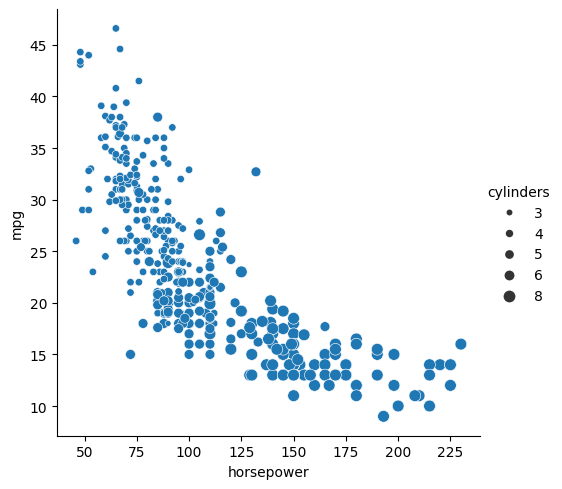
\includegraphics{../images/im268.png}
\end{frame}

\begin{frame}[fragile]{Changing the size of scatter plot points}
\phantomsection\label{changing-the-size-of-scatter-plot-points-7}
\AddToHookNext{env/Highlighting/begin}{\tiny}

\begin{Shaded}
\begin{Highlighting}[]
\CommentTok{\# Create scatter plot of horsepower vs. mpg}
\NormalTok{sns.relplot(x}\OperatorTok{=}\StringTok{"horsepower"}\NormalTok{, y}\OperatorTok{=}\StringTok{"mpg"}\NormalTok{, }
\NormalTok{            data}\OperatorTok{=}\NormalTok{mpg, kind}\OperatorTok{=}\StringTok{"scatter"}\NormalTok{, }
\NormalTok{            size}\OperatorTok{=}\StringTok{"cylinders"}\NormalTok{, hue}\OperatorTok{=}\StringTok{"cylinders"}\NormalTok{)}
\end{Highlighting}
\end{Shaded}
\end{frame}

\begin{frame}{Changing the size of scatter plot points}
\phantomsection\label{changing-the-size-of-scatter-plot-points-8}
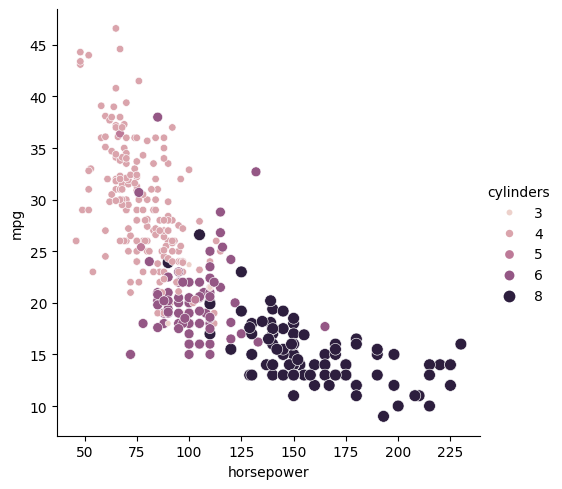
\includegraphics{../images/im269.png}
\end{frame}

\begin{frame}{Changing the style of scatter plot points}
\phantomsection\label{changing-the-style-of-scatter-plot-points}
Let's continue exploring Seaborn's mpg dataset by looking at the
relationship between how fast a car can accelerate (``acceleration'')
and its fuel efficiency (``mpg'').

Do these properties vary by country of origin (``origin'')?
\end{frame}

\begin{frame}{Changing the style of scatter plot points}
\phantomsection\label{changing-the-style-of-scatter-plot-points-1}
Note that the ``acceleration'' variable is the time to accelerate from 0
to 60 miles per hour, in seconds. Higher values indicate slower
acceleration.
\end{frame}

\begin{frame}{Changing the style of scatter plot points}
\phantomsection\label{changing-the-style-of-scatter-plot-points-2}
Use relplot() and the mpg DataFrame to create a scatter plot with
``acceleration'' on the x-axis and ``mpg'' on the y-axis.
\end{frame}

\begin{frame}[fragile]{Changing the style of scatter plot points}
\phantomsection\label{changing-the-style-of-scatter-plot-points-3}
\AddToHookNext{env/Highlighting/begin}{\tiny}

\begin{Shaded}
\begin{Highlighting}[]
\CommentTok{\# Import Matplotlib and Seaborn}
\ImportTok{import}\NormalTok{ matplotlib.pyplot }\ImportTok{as}\NormalTok{ plt}
\ImportTok{import}\NormalTok{ seaborn }\ImportTok{as}\NormalTok{ sns}
\end{Highlighting}
\end{Shaded}
\end{frame}

\begin{frame}{Changing the style of scatter plot points}
\phantomsection\label{changing-the-style-of-scatter-plot-points-4}
Vary the style and color of the plot points by country of origin
(``origin'').
\end{frame}

\begin{frame}[fragile]{Changing the style of scatter plot points}
\phantomsection\label{changing-the-style-of-scatter-plot-points-5}
\AddToHookNext{env/Highlighting/begin}{\tiny}

\begin{Shaded}
\begin{Highlighting}[]
\CommentTok{\# Create a scatter plot of acceleration vs. mpg}
\NormalTok{sns.relplot(x}\OperatorTok{=}\StringTok{"acceleration"}\NormalTok{, y}\OperatorTok{=}\StringTok{"mpg"}\NormalTok{, }
\NormalTok{            data}\OperatorTok{=}\NormalTok{mpg, kind}\OperatorTok{=}\StringTok{"scatter"}\NormalTok{, }
\NormalTok{            style}\OperatorTok{=}\StringTok{"origin"}\NormalTok{, hue}\OperatorTok{=}\StringTok{"origin"}\NormalTok{)}
\end{Highlighting}
\end{Shaded}
\end{frame}

\begin{frame}{Changing the style of scatter plot points}
\phantomsection\label{changing-the-style-of-scatter-plot-points-6}
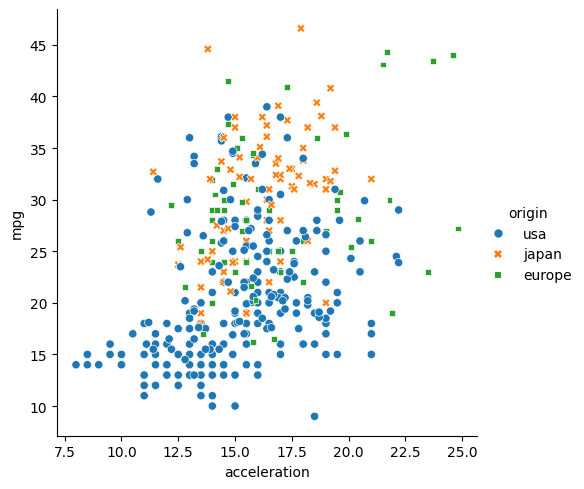
\includegraphics{../images/im270.png}
\end{frame}

\begin{frame}{Interpreting line plots}
\phantomsection\label{interpreting-line-plots}
In this exercise, we'll continue to explore Seaborn's mpg dataset, which
contains one row per car model and includes information such as the year
the car was made, its fuel efficiency (measured in ``miles per gallon''
or ``M.P.G''), and its country of origin (USA, Europe, or Japan).

How has the average miles per gallon achieved by these cars changed over
time? Let's use line plots to find out!
\end{frame}

\begin{frame}[fragile]{Interpreting line plots}
\phantomsection\label{interpreting-line-plots-1}
Use relplot() and the mpg DataFrame to create a line plot with
``model\_year'' on the x-axis and ``mpg'' on the y-axis.

\AddToHookNext{env/Highlighting/begin}{\tiny}

\begin{Shaded}
\begin{Highlighting}[]
\CommentTok{\# Import Matplotlib and Seaborn}
\ImportTok{import}\NormalTok{ matplotlib.pyplot }\ImportTok{as}\NormalTok{ plt}
\ImportTok{import}\NormalTok{ seaborn }\ImportTok{as}\NormalTok{ sns}

\CommentTok{\# Create line plot}
\NormalTok{sns.relplot(x}\OperatorTok{=}\StringTok{"model\_year"}\NormalTok{, y}\OperatorTok{=}\StringTok{"mpg"}\NormalTok{,}
\NormalTok{            data}\OperatorTok{=}\NormalTok{mpg, kind}\OperatorTok{=}\StringTok{"line"}\NormalTok{)}
\end{Highlighting}
\end{Shaded}
\end{frame}

\begin{frame}{Interpreting line plots}
\phantomsection\label{interpreting-line-plots-2}
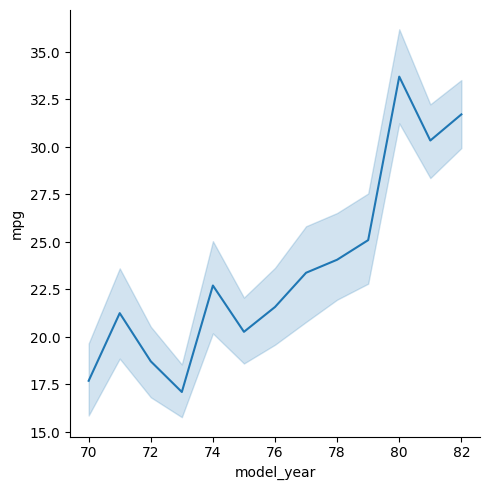
\includegraphics{../images/im271.png}
\end{frame}

\begin{frame}{Visualizing standard deviation with line plots}
\phantomsection\label{visualizing-standard-deviation-with-line-plots}
In the last exercise, we looked at how the average miles per gallon
achieved by cars has changed over time.

Now let's use a line plot to visualize how the distribution of miles per
gallon has changed over time.

Seaborn has been imported as sns and matplotlib.pyplot has been imported
as plt.
\end{frame}

\begin{frame}[fragile]{Visualizing standard deviation with line plots}
\phantomsection\label{visualizing-standard-deviation-with-line-plots-1}
Change the plot so the shaded area shows the standard deviation instead
of the confidence interval for the mean.

\AddToHookNext{env/Highlighting/begin}{\tiny}

\begin{Shaded}
\begin{Highlighting}[]
\CommentTok{\# Make the shaded area show the standard deviation}
\NormalTok{sns.relplot(x}\OperatorTok{=}\StringTok{"model\_year"}\NormalTok{, y}\OperatorTok{=}\StringTok{"mpg"}\NormalTok{,}
\NormalTok{            data}\OperatorTok{=}\NormalTok{mpg, kind}\OperatorTok{=}\StringTok{"line"}\NormalTok{,}
\NormalTok{            ci}\OperatorTok{=}\StringTok{"sd"}\NormalTok{)}
\end{Highlighting}
\end{Shaded}
\end{frame}

\begin{frame}{Visualizing standard deviation with line plots}
\phantomsection\label{visualizing-standard-deviation-with-line-plots-2}
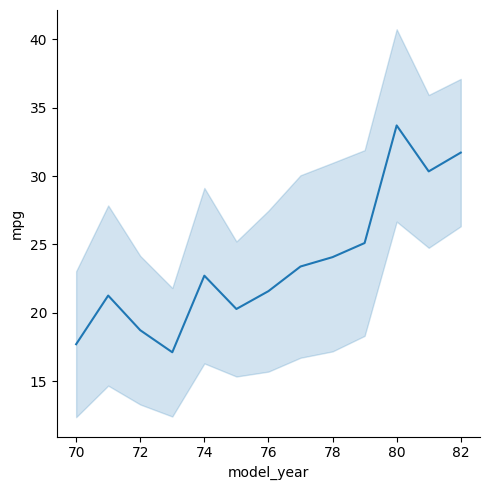
\includegraphics{../images/im272.png}
\end{frame}

\begin{frame}{Plotting subgroups in line plots}
\phantomsection\label{plotting-subgroups-in-line-plots}
Let's continue to look at the mpg dataset. We've seen that the average
miles per gallon for cars has increased over time, but how has the
average horsepower for cars changed over time?

And does this trend differ by country of origin?
\end{frame}

\begin{frame}[fragile]{Plotting subgroups in line plots}
\phantomsection\label{plotting-subgroups-in-line-plots-1}
Use relplot() and the mpg DataFrame to create a line plot with
``model\_year'' on the x-axis and ``horsepower'' on the y-axis. Turn off
the confidence intervals on the plot.

\AddToHookNext{env/Highlighting/begin}{\tiny}

\begin{Shaded}
\begin{Highlighting}[]
\CommentTok{\# Import Matplotlib and Seaborn}
\ImportTok{import}\NormalTok{ matplotlib.pyplot }\ImportTok{as}\NormalTok{ plt}
\ImportTok{import}\NormalTok{ seaborn }\ImportTok{as}\NormalTok{ sns}

\CommentTok{\# Create line plot of model year vs. horsepower}
\NormalTok{sns.relplot(x}\OperatorTok{=}\StringTok{"model\_year"}\NormalTok{, y}\OperatorTok{=}\StringTok{"horsepower"}\NormalTok{, }
\NormalTok{            data}\OperatorTok{=}\NormalTok{mpg, kind}\OperatorTok{=}\StringTok{"line"}\NormalTok{, }
\NormalTok{            ci}\OperatorTok{=}\VariableTok{None}\NormalTok{)}
\end{Highlighting}
\end{Shaded}
\end{frame}

\begin{frame}{Plotting subgroups in line plots}
\phantomsection\label{plotting-subgroups-in-line-plots-2}
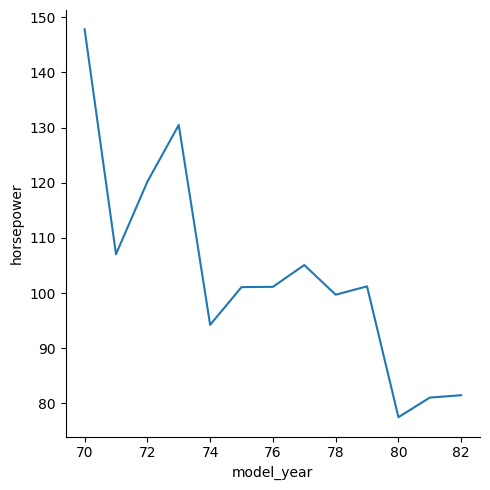
\includegraphics{../images/im273.png}
\end{frame}

\begin{frame}[fragile]{Plotting subgroups in line plots}
\phantomsection\label{plotting-subgroups-in-line-plots-3}
Create different lines for each country of origin (``origin'') that vary
in both line style and color.

\AddToHookNext{env/Highlighting/begin}{\tiny}

\begin{Shaded}
\begin{Highlighting}[]

\end{Highlighting}
\end{Shaded}
\end{frame}

\begin{frame}{Plotting subgroups in line plots}
\phantomsection\label{plotting-subgroups-in-line-plots-4}
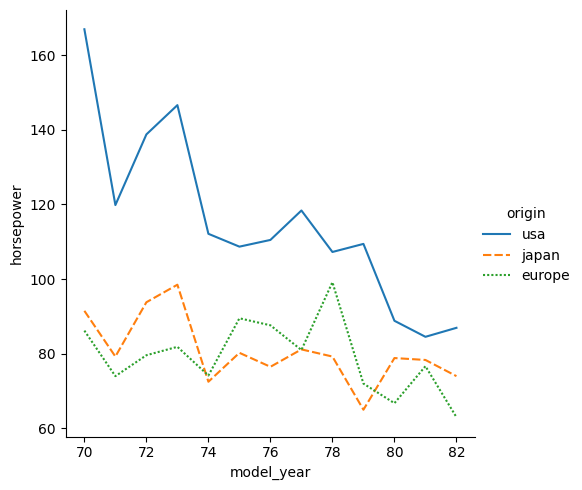
\includegraphics{../images/im275.png}
\end{frame}

\begin{frame}[fragile]{Plotting subgroups in line plots}
\phantomsection\label{plotting-subgroups-in-line-plots-5}
Add markers for each data point to the lines.

\AddToHookNext{env/Highlighting/begin}{\tiny}

\begin{Shaded}
\begin{Highlighting}[]
\CommentTok{\# Change to create subgroups for country of origin}
\NormalTok{sns.relplot(x}\OperatorTok{=}\StringTok{"model\_year"}\NormalTok{, y}\OperatorTok{=}\StringTok{"horsepower"}\NormalTok{, }
\NormalTok{            data}\OperatorTok{=}\NormalTok{mpg, kind}\OperatorTok{=}\StringTok{"line"}\NormalTok{, }
\NormalTok{            ci}\OperatorTok{=}\VariableTok{None}\NormalTok{, style}\OperatorTok{=}\StringTok{"origin"}\NormalTok{, }
\NormalTok{            hue}\OperatorTok{=}\StringTok{"origin"}\NormalTok{)}
\end{Highlighting}
\end{Shaded}
\end{frame}

\begin{frame}{Plotting subgroups in line plots}
\phantomsection\label{plotting-subgroups-in-line-plots-6}
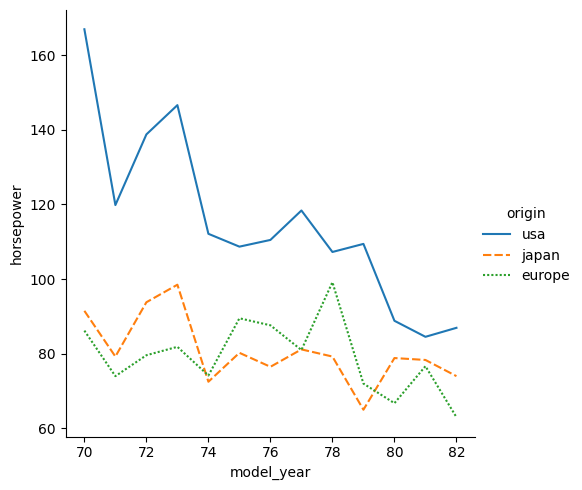
\includegraphics{../images/im275.png}
\end{frame}

\begin{frame}[fragile]{Plotting subgroups in line plots}
\phantomsection\label{plotting-subgroups-in-line-plots-7}
Use the dashes parameter to use solid lines for all countries, while
still allowing for different marker styles for each line.

\AddToHookNext{env/Highlighting/begin}{\tiny}

\begin{Shaded}
\begin{Highlighting}[]
\CommentTok{\# Add markers and make each line have the same style}
\NormalTok{sns.relplot(x}\OperatorTok{=}\StringTok{"model\_year"}\NormalTok{, y}\OperatorTok{=}\StringTok{"horsepower"}\NormalTok{, }
\NormalTok{            data}\OperatorTok{=}\NormalTok{mpg, kind}\OperatorTok{=}\StringTok{"line"}\NormalTok{, }
\NormalTok{            ci}\OperatorTok{=}\VariableTok{None}\NormalTok{, style}\OperatorTok{=}\StringTok{"origin"}\NormalTok{, }
\NormalTok{            hue}\OperatorTok{=}\StringTok{"origin"}\NormalTok{, markers}\OperatorTok{=}\VariableTok{True}\NormalTok{,}
\NormalTok{            dashes}\OperatorTok{=}\VariableTok{False}\NormalTok{)}
\end{Highlighting}
\end{Shaded}
\end{frame}

\begin{frame}{Plotting subgroups in line plots}
\phantomsection\label{plotting-subgroups-in-line-plots-8}
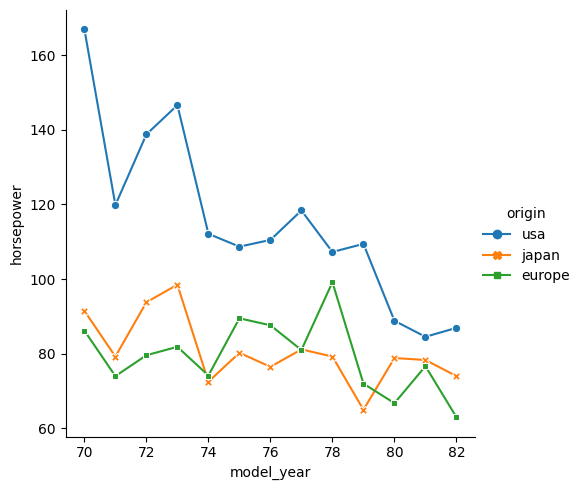
\includegraphics{../images/im276.png}
\end{frame}

\section{Visualizing a Categorical and a Quantitative
Variable}\label{visualizing-a-categorical-and-a-quantitative-variable}

\begin{frame}{Count plots}
\phantomsection\label{count-plots}
In this exercise, we'll return to exploring our dataset that contains
the responses to a survey sent out to young people. We might suspect
that young people spend a lot of time on the internet, but how much do
they report using the internet each day?
\end{frame}

\begin{frame}{Count plots}
\phantomsection\label{count-plots-1}
Let's use a count plot to break down the number of survey responses in
each category and then explore whether it changes based on age.
\end{frame}

\begin{frame}[fragile]{Count plots}
\phantomsection\label{count-plots-2}
As a reminder, to create a count plot, we'll use the catplot() function
and specify the name of the categorical variable to count (x=\_\_\_\_),
the pandas DataFrame to use (data=\_\_\_\_), and the type of plot
(kind=``count'').

\AddToHookNext{env/Highlighting/begin}{\tiny}

\begin{Shaded}
\begin{Highlighting}[]
\ImportTok{import}\NormalTok{ pandas }\ImportTok{as}\NormalTok{ pd}
\ImportTok{import}\NormalTok{ seaborn }\ImportTok{as}\NormalTok{ sns}
\ImportTok{import}\NormalTok{ matplotlib.pyplot }\ImportTok{as}\NormalTok{ plt}

\CommentTok{\# URL for the dataset}
\NormalTok{url }\OperatorTok{=} \StringTok{"https://raw.githubusercontent.com/endri81/DataVisualization/refs/heads/main/data/young{-}people{-}survey{-}responses.csv"}

\CommentTok{\# Load the dataset}
\NormalTok{survey\_data }\OperatorTok{=}\NormalTok{ pd.read\_csv(url)}
\end{Highlighting}
\end{Shaded}
\end{frame}

\begin{frame}[fragile]{Count plots}
\phantomsection\label{count-plots-3}
Use sns.catplot() to create a count plot using the survey\_data
DataFrame with ``Internet usage'' on the x-axis.

\AddToHookNext{env/Highlighting/begin}{\tiny}

\begin{Shaded}
\begin{Highlighting}[]
\CommentTok{\#\# Count plots}
\NormalTok{sns.set\_context(}\StringTok{"paper"}\NormalTok{, font\_scale}\OperatorTok{=}\FloatTok{0.8}\NormalTok{)}
\ImportTok{import}\NormalTok{ numpy }\ImportTok{as}\NormalTok{ np}
\NormalTok{survey\_data }\OperatorTok{=}\NormalTok{ pd.read\_csv(}\StringTok{"young{-}people{-}survey{-}responses.csv"}\NormalTok{)}
\NormalTok{survey\_data[}\StringTok{"Age Category"}\NormalTok{] }\OperatorTok{=}\NormalTok{ np.where(survey\_data[}\StringTok{"Age"}\NormalTok{]}\OperatorTok{\textless{}}\DecValTok{21}\NormalTok{, }\StringTok{"Less than 21"}\NormalTok{, }\StringTok{"21+"}\NormalTok{)}
\CommentTok{\# Create count plot of internet usage}
\NormalTok{sns.catplot(x}\OperatorTok{=}\StringTok{"Internet usage"}\NormalTok{, data}\OperatorTok{=}\NormalTok{survey\_data,}
\NormalTok{            kind}\OperatorTok{=}\StringTok{"count"}\NormalTok{)}
\end{Highlighting}
\end{Shaded}
\end{frame}

\begin{frame}{Count plots}
\phantomsection\label{count-plots-4}
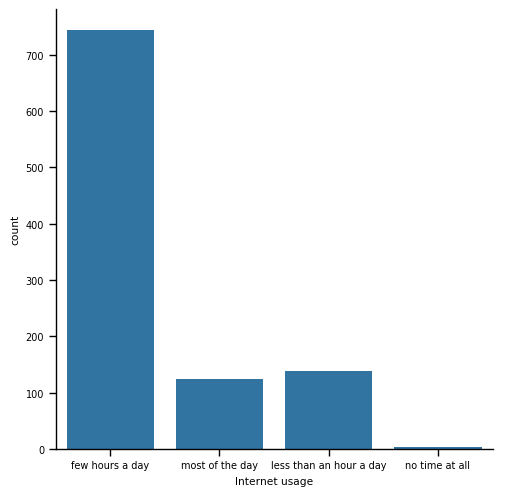
\includegraphics{../images/im278.png}
\end{frame}

\begin{frame}[fragile]{Count plots}
\phantomsection\label{count-plots-5}
Make the bars horizontal instead of vertical.

\AddToHookNext{env/Highlighting/begin}{\tiny}

\begin{Shaded}
\begin{Highlighting}[]
\CommentTok{\# Change the orientation of the plot}
\NormalTok{sns.catplot(y}\OperatorTok{=}\StringTok{"Internet usage"}\NormalTok{, data}\OperatorTok{=}\NormalTok{survey\_data,}
\NormalTok{            kind}\OperatorTok{=}\StringTok{"count"}\NormalTok{)}
\end{Highlighting}
\end{Shaded}
\end{frame}

\begin{frame}{Count plots}
\phantomsection\label{count-plots-6}
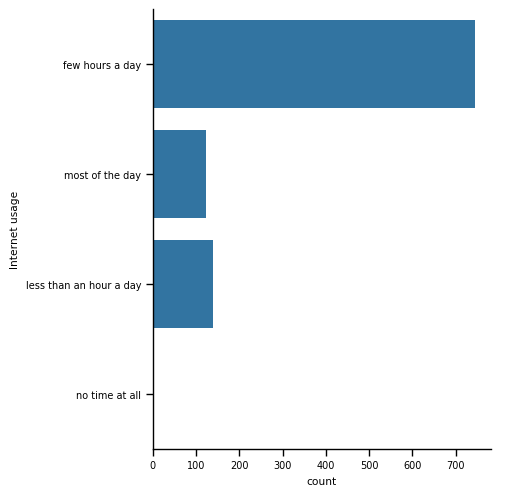
\includegraphics{../images/im279.png}
\end{frame}

\begin{frame}[fragile]{Count plots}
\phantomsection\label{count-plots-7}
Separate this plot into two side-by-side column subplots based on ``Age
Category'', which separates respondents into those that are younger than
21 vs.~21 and older.

\AddToHookNext{env/Highlighting/begin}{\tiny}

\begin{Shaded}
\begin{Highlighting}[]
\CommentTok{\# Separate into column subplots based on age category}
\NormalTok{sns.catplot(y}\OperatorTok{=}\StringTok{"Internet usage"}\NormalTok{, data}\OperatorTok{=}\NormalTok{survey\_data,}
\NormalTok{            kind}\OperatorTok{=}\StringTok{"count"}\NormalTok{, col}\OperatorTok{=}\StringTok{"Age Category"}\NormalTok{)}
\end{Highlighting}
\end{Shaded}
\end{frame}

\begin{frame}{Count plots}
\phantomsection\label{count-plots-8}
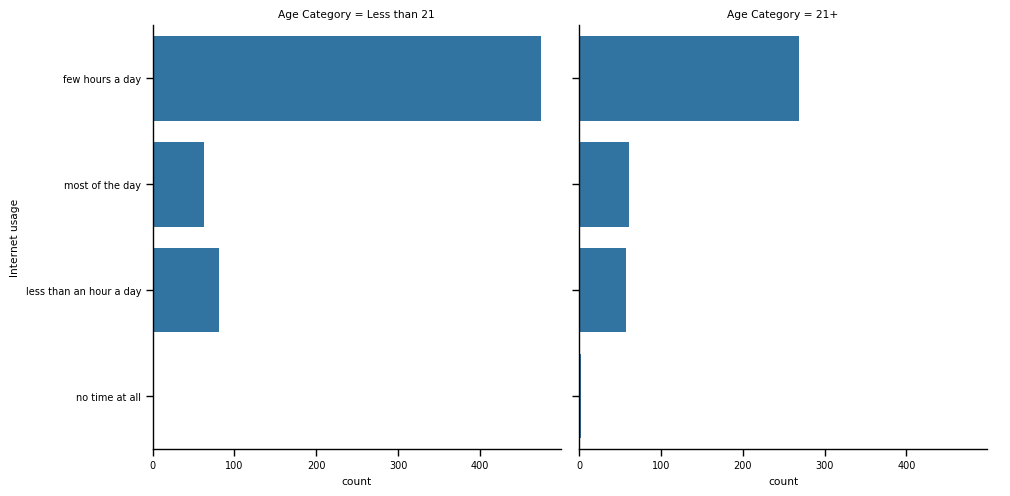
\includegraphics{../images/im280.png}
\end{frame}

\begin{frame}{Bar plots with percentages}
\phantomsection\label{bar-plots-with-percentages}
Let's continue exploring the responses to a survey sent out to young
people.

The variable ``Interested in Math'' is True if the person reported being
interested or very interested in mathematics, and False otherwise.
\end{frame}

\begin{frame}{Bar plots with percentages}
\phantomsection\label{bar-plots-with-percentages-1}
What percentage of young people report being interested in math, and
does this vary based on gender? Let's use a bar plot to find out.
\end{frame}

\begin{frame}{Bar plots with percentages}
\phantomsection\label{bar-plots-with-percentages-2}
As a reminder, we'll create a bar plot using the catplot() function,
providing the name of categorical variable to put on the x-axis
(x=\_\_\_\_), the name of the quantitative variable to summarize on the
y-axis (y=\_\_\_\_), the pandas DataFrame to use (data=\_\_\_\_), and
the type of categorical plot (kind=``bar'').
\end{frame}

\begin{frame}{Bar plots with percentages}
\phantomsection\label{bar-plots-with-percentages-3}
Use the survey\_data DataFrame and sns.catplot() to create a bar plot
with ``Gender'' on the x-axis and ``Interested in Math'' on the y-axis.
\end{frame}

\begin{frame}[fragile]{Bar plots with percentages}
\phantomsection\label{bar-plots-with-percentages-4}
\AddToHookNext{env/Highlighting/begin}{\tiny}

\begin{Shaded}
\begin{Highlighting}[]
\NormalTok{sns.reset\_defaults()}
\CommentTok{\# Ensure the column names match exactly}
\NormalTok{gender\_col }\OperatorTok{=} \StringTok{"Gender"}
\NormalTok{math\_interest\_col }\OperatorTok{=} \StringTok{"Interested in Math"}
\end{Highlighting}
\end{Shaded}
\end{frame}

\begin{frame}[fragile]{Bar plots with percentages}
\phantomsection\label{bar-plots-with-percentages-5}
\AddToHookNext{env/Highlighting/begin}{\tiny}

\begin{Shaded}
\begin{Highlighting}[]
\CommentTok{\# Drop missing values if necessary}
\NormalTok{survey\_data }\OperatorTok{=}\NormalTok{ survey\_data.dropna(subset}\OperatorTok{=}\NormalTok{[math\_interest\_col])}
\CommentTok{\# Convert to numeric if needed}
\NormalTok{survey\_data[math\_interest\_col] }\OperatorTok{=}\NormalTok{ pd.to\_numeric(survey\_data[math\_interest\_col], errors}\OperatorTok{=}\StringTok{"coerce"}\NormalTok{)}
\CommentTok{\# Create the bar plot}
\NormalTok{sns.catplot(x}\OperatorTok{=}\NormalTok{gender\_col, y}\OperatorTok{=}\NormalTok{math\_interest\_col, data}\OperatorTok{=}\NormalTok{survey\_data, kind}\OperatorTok{=}\StringTok{"bar"}\NormalTok{)}
\end{Highlighting}
\end{Shaded}
\end{frame}

\begin{frame}{Bar plots with percentages}
\phantomsection\label{bar-plots-with-percentages-6}
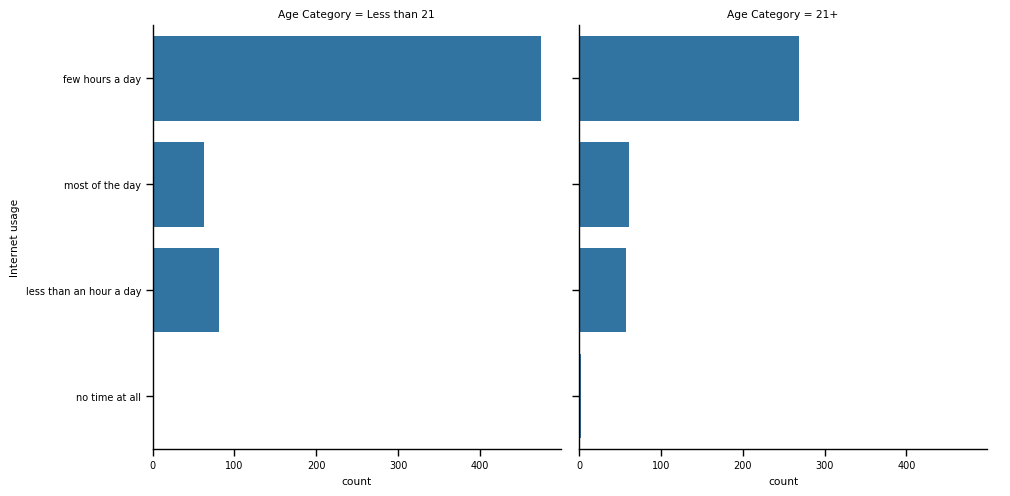
\includegraphics{../images/im281.png}
\end{frame}

\begin{frame}{Customizing bar plots}
\phantomsection\label{customizing-bar-plots}
In this exercise, we'll explore data from students in secondary school.

The ``study\_time'' variable records each student's reported weekly
study time as one of the following categories: ``\textless2 hours'', ``2
to 5 hours'', ``5 to 10 hours'', or ``\textgreater10 hours''.
\end{frame}

\begin{frame}[fragile]{Customizing bar plots}
\phantomsection\label{customizing-bar-plots-1}
Do students who report higher amounts of studying tend to get better
final grades?

\AddToHookNext{env/Highlighting/begin}{\tiny}

\begin{Shaded}
\begin{Highlighting}[]
\ImportTok{import}\NormalTok{ pandas }\ImportTok{as}\NormalTok{ pd}
\ImportTok{import}\NormalTok{ seaborn }\ImportTok{as}\NormalTok{ sns}
\ImportTok{import}\NormalTok{ matplotlib.pyplot }\ImportTok{as}\NormalTok{ plt}

\CommentTok{\# URL for the dataset}
\NormalTok{url }\OperatorTok{=} \StringTok{"https://raw.githubusercontent.com/endri81/DataVisualization/refs/heads/main/data/student{-}alcohol{-}consumption.csv"}

\CommentTok{\# Load the dataset}
\NormalTok{student\_data }\OperatorTok{=}\NormalTok{ pd.read\_csv(url)}
\end{Highlighting}
\end{Shaded}
\end{frame}

\begin{frame}{Customizing bar plots}
\phantomsection\label{customizing-bar-plots-2}
Let's compare the average final grade among students in each category
using a bar plot.
\end{frame}

\begin{frame}[fragile]{Customizing bar plots}
\phantomsection\label{customizing-bar-plots-3}
Use sns.catplot() to create a bar plot with ``study\_time'' on the
x-axis and final grade (``G3'') on the y-axis, using the student\_data
DataFrame.

\AddToHookNext{env/Highlighting/begin}{\tiny}

\begin{Shaded}
\begin{Highlighting}[]
\CommentTok{\# Drop missing values in final grade}
\NormalTok{student\_data }\OperatorTok{=}\NormalTok{ student\_data.dropna(subset}\OperatorTok{=}\NormalTok{[final\_grade\_col])}

\CommentTok{\# Convert study\_time to categorical if needed}
\NormalTok{student\_data[study\_time\_col] }\OperatorTok{=}\NormalTok{ student\_data[study\_time\_col].astype(}\BuiltInTok{str}\NormalTok{)}

\CommentTok{\# Set seaborn context}
\NormalTok{sns.set\_context(}\StringTok{"paper"}\NormalTok{, font\_scale}\OperatorTok{=}\FloatTok{0.8}\NormalTok{)}

\CommentTok{\# Create bar plot}
\NormalTok{sns.catplot(x}\OperatorTok{=}\NormalTok{study\_time\_col, y}\OperatorTok{=}\NormalTok{final\_grade\_col, }
\NormalTok{            data}\OperatorTok{=}\NormalTok{student\_data, kind}\OperatorTok{=}\StringTok{"bar"}\NormalTok{)}

\CommentTok{\# Show the plot}
\NormalTok{plt.show()}
\end{Highlighting}
\end{Shaded}
\end{frame}

\begin{frame}{Customizing bar plots}
\phantomsection\label{customizing-bar-plots-4}
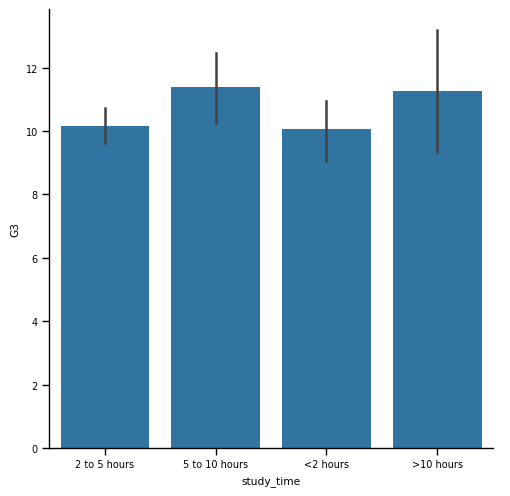
\includegraphics{../images/im283.png}
\end{frame}

\begin{frame}[fragile]{Customizing bar plots}
\phantomsection\label{customizing-bar-plots-5}
Using the order parameter and the category\_order list that is provided,
rearrange the bars so that they are in order from lowest study time to
highest.

\AddToHookNext{env/Highlighting/begin}{\tiny}

\begin{Shaded}
\begin{Highlighting}[]
\CommentTok{\# List of categories from lowest to highest}
\NormalTok{category\_order }\OperatorTok{=}\NormalTok{ [}\StringTok{"\textless{}2 hours"}\NormalTok{, }
                  \StringTok{"2 to 5 hours"}\NormalTok{, }
                  \StringTok{"5 to 10 hours"}\NormalTok{, }
                  \StringTok{"\textgreater{}10 hours"}\NormalTok{]}

\CommentTok{\# Rearrange the categories}
\NormalTok{sns.catplot(x}\OperatorTok{=}\StringTok{"study\_time"}\NormalTok{, y}\OperatorTok{=}\StringTok{"G3"}\NormalTok{,}
\NormalTok{            data}\OperatorTok{=}\NormalTok{student\_data,}
\NormalTok{            kind}\OperatorTok{=}\StringTok{"bar"}\NormalTok{,}
\NormalTok{            order}\OperatorTok{=}\NormalTok{category\_order)}
\end{Highlighting}
\end{Shaded}
\end{frame}

\begin{frame}{Customizing bar plots}
\phantomsection\label{customizing-bar-plots-6}
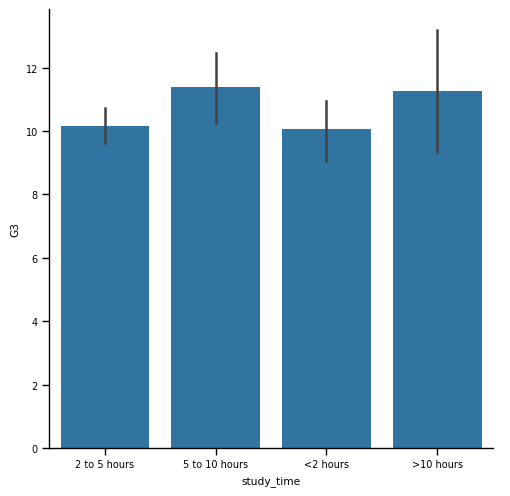
\includegraphics{../images/im283.png}
\end{frame}

\begin{frame}[fragile]{Customizing bar plots}
\phantomsection\label{customizing-bar-plots-7}
Update the plot so that it no longer displays confidence intervals.

\AddToHookNext{env/Highlighting/begin}{\tiny}

\begin{Shaded}
\begin{Highlighting}[]
\CommentTok{\# List of categories from lowest to highest}
\NormalTok{category\_order }\OperatorTok{=}\NormalTok{ [}\StringTok{"\textless{}2 hours"}\NormalTok{, }
                  \StringTok{"2 to 5 hours"}\NormalTok{, }
                  \StringTok{"5 to 10 hours"}\NormalTok{, }
                  \StringTok{"\textgreater{}10 hours"}\NormalTok{]}

\CommentTok{\# Create bar plot with the correct parameter}
\NormalTok{sns.catplot(x}\OperatorTok{=}\NormalTok{study\_time\_col, y}\OperatorTok{=}\NormalTok{final\_grade\_col, }
\NormalTok{            data}\OperatorTok{=}\NormalTok{student\_data, kind}\OperatorTok{=}\StringTok{"bar"}\NormalTok{, errorbar}\OperatorTok{=}\VariableTok{None}\NormalTok{)}

\CommentTok{\# Show the plot}
\NormalTok{plt.show()}
\end{Highlighting}
\end{Shaded}
\end{frame}

\begin{frame}{Customizing bar plots}
\phantomsection\label{customizing-bar-plots-8}
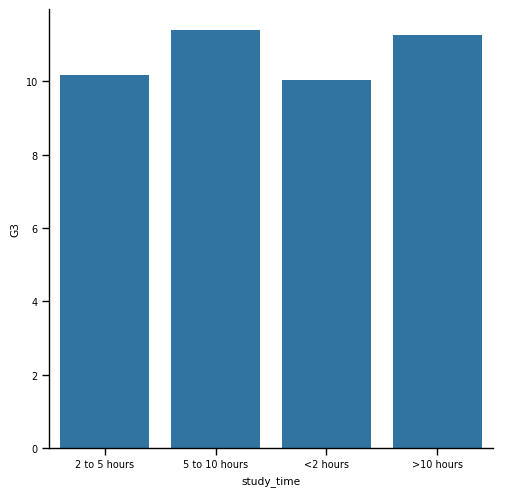
\includegraphics{../images/im284.png}
\end{frame}

\begin{frame}{Create and interpret a box plot}
\phantomsection\label{create-and-interpret-a-box-plot}
Let's continue using the student\_data dataset.

In an earlier exercise, we explored the relationship between studying
and final grade by using a bar plot to compare the average final grade
(``G3'') among students in different categories of ``study\_time''.
\end{frame}

\begin{frame}{Create and interpret a box plot}
\phantomsection\label{create-and-interpret-a-box-plot-1}
In this exercise, we'll try using a box plot look at this relationship
instead.

As a reminder, to create a box plot you'll need to use the catplot()
function and specify the name of the categorical variable to put on the
x-axis (x=\_\_\_\_), the name of the quantitative variable to summarize
on the y-axis (y=\_\_\_\_), the pandas DataFrame to use (data=\_\_\_\_),
and the type of plot (kind=``box'').
\end{frame}

\begin{frame}{Create and interpret a box plot}
\phantomsection\label{create-and-interpret-a-box-plot-2}
Use sns.catplot() and the student\_data DataFrame to create a box plot
with ``study\_time'' on the x-axis and ``G3'' on the y-axis.

Set the ordering of the categories to study\_time\_order.
\end{frame}

\begin{frame}[fragile]{Create and interpret a box plot}
\phantomsection\label{create-and-interpret-a-box-plot-3}
\AddToHookNext{env/Highlighting/begin}{\tiny}

\begin{Shaded}
\begin{Highlighting}[]
\CommentTok{\#\# Create and interpret a box plot}

\CommentTok{\# Specify the category ordering}
\NormalTok{study\_time\_order }\OperatorTok{=}\NormalTok{ [}\StringTok{"\textless{}2 hours"}\NormalTok{, }\StringTok{"2 to 5 hours"}\NormalTok{, }
                    \StringTok{"5 to 10 hours"}\NormalTok{, }\StringTok{"\textgreater{}10 hours"}\NormalTok{]}

\CommentTok{\# Create a box plot and set the order of the categories}
\NormalTok{sns.catplot(x}\OperatorTok{=}\StringTok{"study\_time"}\NormalTok{, y}\OperatorTok{=}\StringTok{"G3"}\NormalTok{,}
\NormalTok{            data}\OperatorTok{=}\NormalTok{student\_data,}
\NormalTok{            kind}\OperatorTok{=}\StringTok{"box"}\NormalTok{,}
\NormalTok{            order}\OperatorTok{=}\NormalTok{study\_time\_order)}
\end{Highlighting}
\end{Shaded}
\end{frame}

\begin{frame}{Create and interpret a box plot}
\phantomsection\label{create-and-interpret-a-box-plot-4}
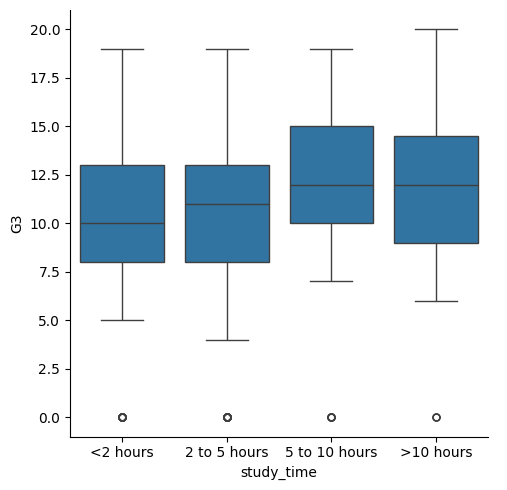
\includegraphics{../images/im285.png}
\end{frame}

\begin{frame}{Omitting outliers}
\phantomsection\label{omitting-outliers}
Now let's use the student\_data dataset to compare the distribution of
final grades (``G3'') between students who have internet access at home
and those who don't.

To do this, we'll use the ``internet'' variable, which is a binary
(yes/no) indicator of whether the student has internet access at home.
\end{frame}

\begin{frame}{Omitting outliers}
\phantomsection\label{omitting-outliers-1}
Since internet may be less accessible in rural areas, we'll add
subgroups based on where the student lives.

For this, we can use the ``location'' variable, which is an indicator of
whether a student lives in an urban (``Urban'') or rural (``Rural'')
location.
\end{frame}

\begin{frame}{Omitting outliers}
\phantomsection\label{omitting-outliers-2}
Use sns.catplot() to create a box plot with the student\_data DataFrame,
putting ``internet'' on the x-axis and ``G3'' on the y-axis.

Add subgroups so each box plot is colored based on ``location''.

Do not display the outliers.
\end{frame}

\begin{frame}[fragile]{Omitting outliers}
\phantomsection\label{omitting-outliers-3}
\AddToHookNext{env/Highlighting/begin}{\tiny}

\begin{Shaded}
\begin{Highlighting}[]
\CommentTok{\# Create a box plot with subgroups and omit the outliers}
\NormalTok{sns.catplot(x}\OperatorTok{=}\StringTok{"internet"}\NormalTok{, y}\OperatorTok{=}\StringTok{"G3"}\NormalTok{,}
\NormalTok{            data}\OperatorTok{=}\NormalTok{student\_data,}
\NormalTok{            kind}\OperatorTok{=}\StringTok{"box"}\NormalTok{,}
\NormalTok{            hue}\OperatorTok{=}\StringTok{"location"}\NormalTok{,}
\NormalTok{            flierprops}\OperatorTok{=}\NormalTok{\{}\StringTok{"marker"}\NormalTok{: }\StringTok{""}\NormalTok{\})  }
\end{Highlighting}
\end{Shaded}
\end{frame}

\begin{frame}{Omitting outliers}
\phantomsection\label{omitting-outliers-4}
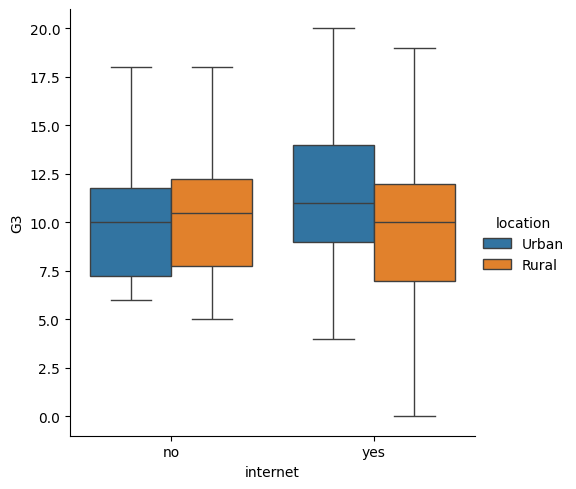
\includegraphics{../images/im286.png}
\end{frame}

\begin{frame}{Adjusting the whiskers}
\phantomsection\label{adjusting-the-whiskers}
In the lesson we saw that there are multiple ways to define the whiskers
in a box plot.

In this set of exercises, we'll continue to use the student\_data
dataset to compare the distribution of final grades (``G3'') between
students who are in a romantic relationship and those that are not.
\end{frame}

\begin{frame}{Adjusting the whiskers}
\phantomsection\label{adjusting-the-whiskers-1}
We'll use the ``romantic'' variable, which is a yes/no indicator of
whether the student is in a romantic relationship.

Let's create a box plot to look at this relationship and try different
ways to define the whiskers.
\end{frame}

\begin{frame}{Adjusting the whiskers}
\phantomsection\label{adjusting-the-whiskers-2}
Adjust the code to make the box plot whiskers to extend to 0.5 * IQR.
Recall: the IQR is the interquartile range.

Change the code to set the whiskers to extend to the 5th and 95th
percentiles.

Change the code to set the whiskers to extend to the min and max values.
\end{frame}

\begin{frame}[fragile]{Adjusting the whiskers}
\phantomsection\label{adjusting-the-whiskers-3}
\AddToHookNext{env/Highlighting/begin}{\tiny}

\begin{Shaded}
\begin{Highlighting}[]
\CommentTok{\# Set the whiskers to 0.5 * IQR}
\NormalTok{sns.catplot(x}\OperatorTok{=}\StringTok{"romantic"}\NormalTok{, y}\OperatorTok{=}\StringTok{"G3"}\NormalTok{,}
\NormalTok{            data}\OperatorTok{=}\NormalTok{student\_data,}
\NormalTok{            kind}\OperatorTok{=}\StringTok{"box"}\NormalTok{,}
\NormalTok{            whis}\OperatorTok{=}\FloatTok{0.5}\NormalTok{)}
\end{Highlighting}
\end{Shaded}
\end{frame}

\begin{frame}{Adjusting the whiskers}
\phantomsection\label{adjusting-the-whiskers-4}
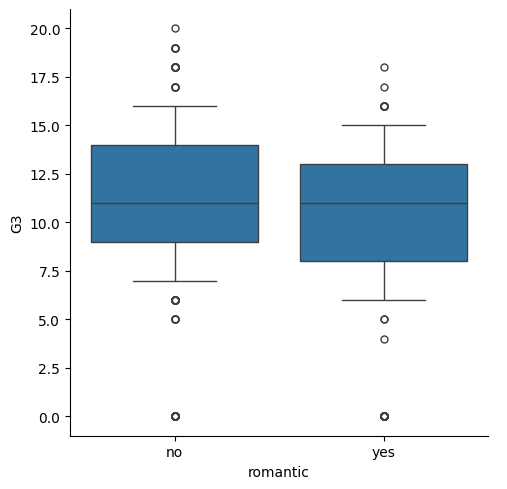
\includegraphics{../images/im287.png}
\end{frame}

\begin{frame}[fragile]{Adjusting the whiskers}
\phantomsection\label{adjusting-the-whiskers-5}
\AddToHookNext{env/Highlighting/begin}{\tiny}

\begin{Shaded}
\begin{Highlighting}[]
\CommentTok{\# Extend the whiskers to the 5th and 95th percentile}
\NormalTok{sns.catplot(x}\OperatorTok{=}\StringTok{"romantic"}\NormalTok{, y}\OperatorTok{=}\StringTok{"G3"}\NormalTok{,}
\NormalTok{            data}\OperatorTok{=}\NormalTok{student\_data,}
\NormalTok{            kind}\OperatorTok{=}\StringTok{"box"}\NormalTok{,}
\NormalTok{            whis}\OperatorTok{=}\NormalTok{[}\DecValTok{5}\NormalTok{, }\DecValTok{95}\NormalTok{])}
\end{Highlighting}
\end{Shaded}
\end{frame}

\begin{frame}{Adjusting the whiskers}
\phantomsection\label{adjusting-the-whiskers-6}
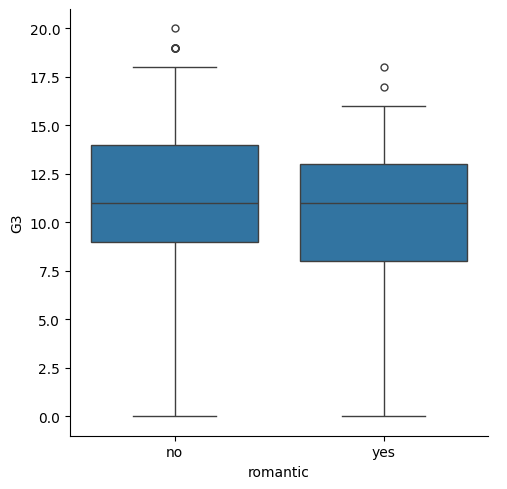
\includegraphics{../images/im288.png}
\end{frame}

\begin{frame}[fragile]{Adjusting the whiskers}
\phantomsection\label{adjusting-the-whiskers-7}
\AddToHookNext{env/Highlighting/begin}{\tiny}

\begin{Shaded}
\begin{Highlighting}[]
\CommentTok{\# Set the whiskers at the min and max values}
\NormalTok{sns.catplot(x}\OperatorTok{=}\StringTok{"romantic"}\NormalTok{, y}\OperatorTok{=}\StringTok{"G3"}\NormalTok{,}
\NormalTok{            data}\OperatorTok{=}\NormalTok{student\_data,}
\NormalTok{            kind}\OperatorTok{=}\StringTok{"box"}\NormalTok{,}
\NormalTok{            whis}\OperatorTok{=}\NormalTok{[}\DecValTok{0}\NormalTok{, }\DecValTok{100}\NormalTok{])}
\end{Highlighting}
\end{Shaded}
\end{frame}

\begin{frame}{Adjusting the whiskers}
\phantomsection\label{adjusting-the-whiskers-8}
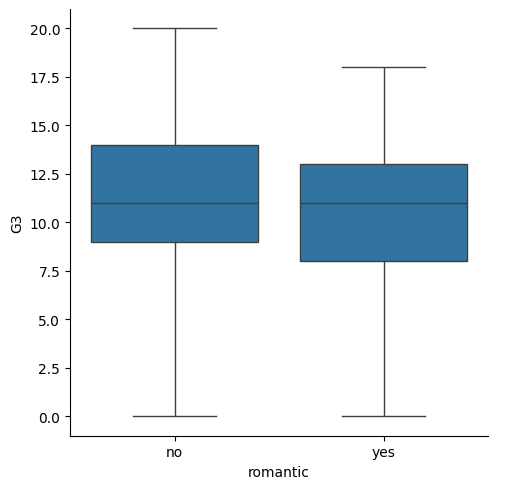
\includegraphics{../images/im289.png}
\end{frame}

\begin{frame}{Customizing point plots}
\phantomsection\label{customizing-point-plots}
Let's continue to look at data from students in secondary school, this
time using a point plot to answer the question: does the quality of the
student's family relationship influence the number of absences the
student has in school?
\end{frame}

\begin{frame}{Customizing point plots}
\phantomsection\label{customizing-point-plots-1}
Here, we'll use the ``famrel'' variable, which describes the quality of
a student's family relationship from 1 (very bad) to 5 (very good).
\end{frame}

\begin{frame}{Customizing point plots}
\phantomsection\label{customizing-point-plots-2}
As a reminder, to create a point plot, use the catplot() function and
specify the name of the categorical variable to put on the x-axis
(x=\_\_\_\_), the name of the quantitative variable to summarize on the
y-axis (y=\_\_\_\_), the pandas DataFrame to use (data=\_\_\_\_), and
the type of categorical plot (kind=``point'').
\end{frame}

\begin{frame}{Customizing point plots}
\phantomsection\label{customizing-point-plots-3}
Use sns.catplot() and the student\_data DataFrame to create a point plot
with ``famrel'' on the x-axis and number of absences (``absences'') on
the y-axis.

Add ``caps'' to the end of the confidence intervals with size 0.2.

Remove the lines joining the points in each category.
\end{frame}

\begin{frame}[fragile]{Customizing point plots}
\phantomsection\label{customizing-point-plots-4}
\AddToHookNext{env/Highlighting/begin}{\tiny}

\begin{Shaded}
\begin{Highlighting}[]
\CommentTok{\# Create a point plot of family relationship vs. absences}
\NormalTok{sns.catplot(x}\OperatorTok{=}\StringTok{"famrel"}\NormalTok{, y}\OperatorTok{=}\StringTok{"absences"}\NormalTok{,}
\NormalTok{            data}\OperatorTok{=}\NormalTok{student\_data,}
\NormalTok{            kind}\OperatorTok{=}\StringTok{"point"}\NormalTok{)}
\end{Highlighting}
\end{Shaded}
\end{frame}

\begin{frame}{Customizing point plots}
\phantomsection\label{customizing-point-plots-5}
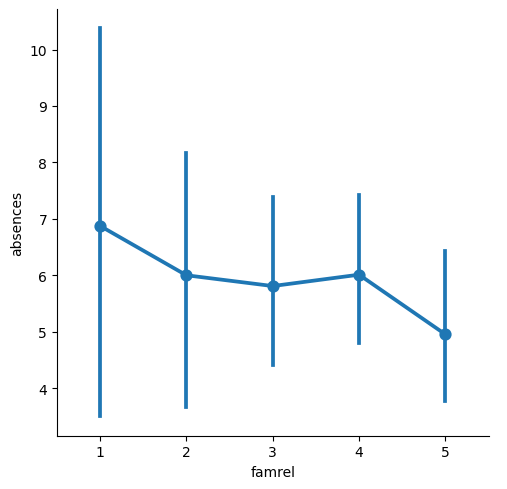
\includegraphics{../images/im290.png}
\end{frame}

\begin{frame}[fragile]{Customizing point plots}
\phantomsection\label{customizing-point-plots-6}
\AddToHookNext{env/Highlighting/begin}{\tiny}

\begin{Shaded}
\begin{Highlighting}[]
\CommentTok{\# Add caps to the confidence interval}
\NormalTok{sns.catplot(x}\OperatorTok{=}\StringTok{"famrel"}\NormalTok{, y}\OperatorTok{=}\StringTok{"absences"}\NormalTok{,}
\NormalTok{            data}\OperatorTok{=}\NormalTok{student\_data,}
\NormalTok{            kind}\OperatorTok{=}\StringTok{"point"}\NormalTok{,}
\NormalTok{            capsize}\OperatorTok{=}\FloatTok{0.2}\NormalTok{)}
\end{Highlighting}
\end{Shaded}
\end{frame}

\begin{frame}{Customizing point plots}
\phantomsection\label{customizing-point-plots-7}
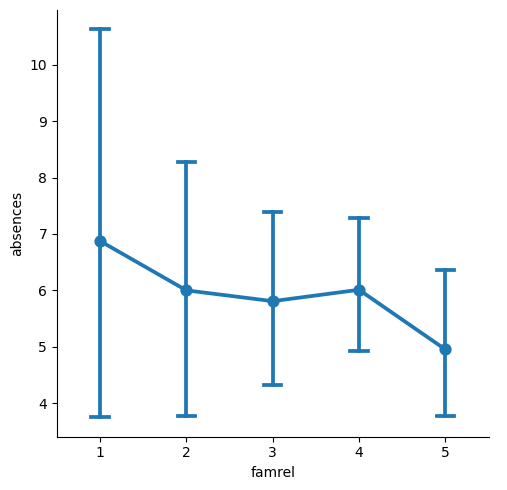
\includegraphics{../images/im291.png}
\end{frame}

\begin{frame}[fragile]{Customizing point plots}
\phantomsection\label{customizing-point-plots-8}
\AddToHookNext{env/Highlighting/begin}{\tiny}

\begin{Shaded}
\begin{Highlighting}[]
\CommentTok{\# Remove the lines joining the points}
\NormalTok{sns.catplot(x}\OperatorTok{=}\StringTok{"famrel"}\NormalTok{, y}\OperatorTok{=}\StringTok{"absences"}\NormalTok{,}
\NormalTok{            data}\OperatorTok{=}\NormalTok{student\_data,}
\NormalTok{            kind}\OperatorTok{=}\StringTok{"point"}\NormalTok{,}
\NormalTok{            capsize}\OperatorTok{=}\FloatTok{0.2}\NormalTok{,}
\NormalTok{            join}\OperatorTok{=}\VariableTok{False}\NormalTok{)}
\end{Highlighting}
\end{Shaded}
\end{frame}

\begin{frame}{Customizing point plots}
\phantomsection\label{customizing-point-plots-9}
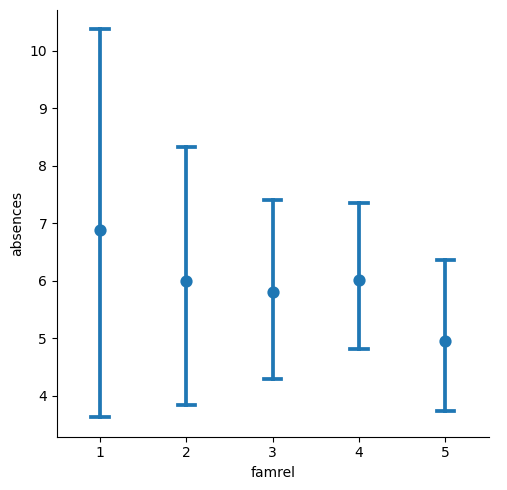
\includegraphics{../images/im292.png}
\end{frame}

\begin{frame}{Point plots with subgroups}
\phantomsection\label{point-plots-with-subgroups}
Let's continue exploring the dataset of students in secondary school.

This time, we'll ask the question: is being in a romantic relationship
associated with higher or lower school attendance?
\end{frame}

\begin{frame}{Point plots with subgroups}
\phantomsection\label{point-plots-with-subgroups-1}
And does this association differ by which school the students attend?
Let's find out using a point plot.
\end{frame}

\begin{frame}{Point plots with subgroups}
\phantomsection\label{point-plots-with-subgroups-2}
Use sns.catplot() and the student\_data DataFrame to create a point plot
with relationship status (``romantic'') on the x-axis and number of
absences (``absences'') on the y-axis.
\end{frame}

\begin{frame}[fragile]{Point plots with subgroups}
\phantomsection\label{point-plots-with-subgroups-3}
\AddToHookNext{env/Highlighting/begin}{\tiny}

\begin{Shaded}
\begin{Highlighting}[]

\end{Highlighting}
\end{Shaded}
\end{frame}

\begin{frame}{Customizing point plots}
\phantomsection\label{customizing-point-plots-10}
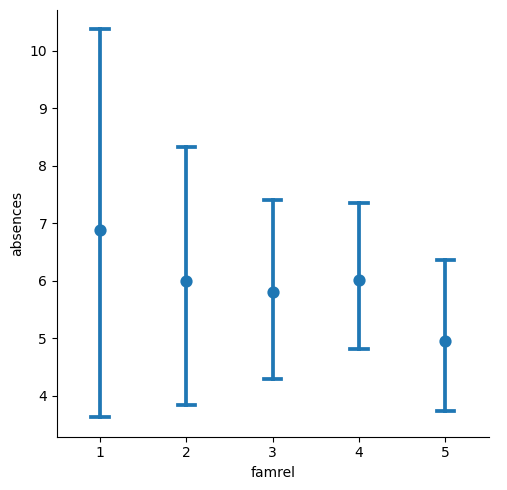
\includegraphics{../images/im292.png}
\end{frame}

\begin{frame}{Point plots with subgroups}
\phantomsection\label{point-plots-with-subgroups-4}
Color the points based on the school that they attend (``school'').
\end{frame}

\begin{frame}[fragile]{Point plots with subgroups}
\phantomsection\label{point-plots-with-subgroups-5}
\AddToHookNext{env/Highlighting/begin}{\tiny}

\begin{Shaded}
\begin{Highlighting}[]
\CommentTok{\# Create a point plot that uses color to create subgroups}
\NormalTok{sns.catplot(x}\OperatorTok{=}\StringTok{"romantic"}\NormalTok{, y}\OperatorTok{=}\StringTok{"absences"}\NormalTok{,}
\NormalTok{            data}\OperatorTok{=}\NormalTok{student\_data,}
\NormalTok{            kind}\OperatorTok{=}\StringTok{"point"}\NormalTok{,}
\NormalTok{            hue}\OperatorTok{=}\StringTok{"school"}\NormalTok{)}
\end{Highlighting}
\end{Shaded}
\end{frame}

\begin{frame}{Customizing point plots}
\phantomsection\label{customizing-point-plots-11}
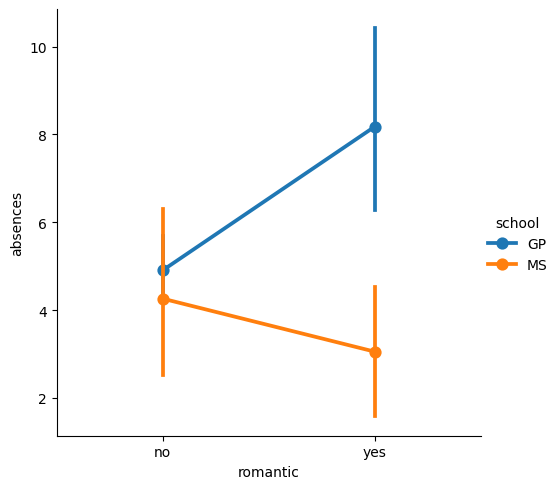
\includegraphics{../images/im293.png}
\end{frame}

\begin{frame}{Point plots with subgroups}
\phantomsection\label{point-plots-with-subgroups-6}
Turn off the confidence intervals for the plot.
\end{frame}

\begin{frame}[fragile]{Point plots with subgroups}
\phantomsection\label{point-plots-with-subgroups-7}
\AddToHookNext{env/Highlighting/begin}{\tiny}

\begin{Shaded}
\begin{Highlighting}[]
\CommentTok{\# Turn off the confidence intervals for this plot}
\NormalTok{sns.catplot(x}\OperatorTok{=}\StringTok{"romantic"}\NormalTok{, y}\OperatorTok{=}\StringTok{"absences"}\NormalTok{,}
\NormalTok{            data}\OperatorTok{=}\NormalTok{student\_data,}
\NormalTok{            kind}\OperatorTok{=}\StringTok{"point"}\NormalTok{,}
\NormalTok{            hue}\OperatorTok{=}\StringTok{"school"}\NormalTok{,}
\NormalTok{            ci}\OperatorTok{=}\VariableTok{None}\NormalTok{)}
\end{Highlighting}
\end{Shaded}
\end{frame}

\begin{frame}{Customizing point plots}
\phantomsection\label{customizing-point-plots-12}
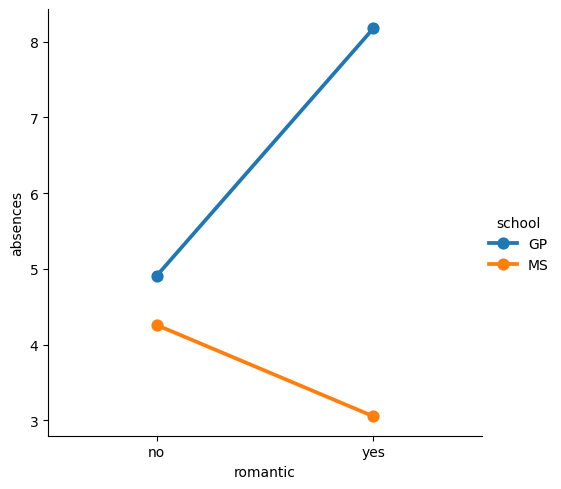
\includegraphics{../images/im294.png}
\end{frame}

\begin{frame}{Point plots with subgroups}
\phantomsection\label{point-plots-with-subgroups-8}
Since there may be outliers of students with many absences, use the
median function that we've imported from numpy to display the median
number of absences instead of the average.
\end{frame}

\begin{frame}[fragile]{Point plots with subgroups}
\phantomsection\label{point-plots-with-subgroups-9}
\AddToHookNext{env/Highlighting/begin}{\tiny}

\begin{Shaded}
\begin{Highlighting}[]
\CommentTok{\# Import median function from numpy}
\ImportTok{from}\NormalTok{ numpy }\ImportTok{import}\NormalTok{ median}

\CommentTok{\# Plot the median number of absences instead of the mean}
\NormalTok{sns.catplot(x}\OperatorTok{=}\StringTok{"romantic"}\NormalTok{, y}\OperatorTok{=}\StringTok{"absences"}\NormalTok{,}
\NormalTok{            data}\OperatorTok{=}\NormalTok{student\_data,}
\NormalTok{            kind}\OperatorTok{=}\StringTok{"point"}\NormalTok{,}
\NormalTok{            hue}\OperatorTok{=}\StringTok{"school"}\NormalTok{,}
\NormalTok{            ci}\OperatorTok{=}\VariableTok{None}\NormalTok{,}
\NormalTok{            estimator}\OperatorTok{=}\NormalTok{median)}
\end{Highlighting}
\end{Shaded}
\end{frame}

\begin{frame}{Customizing point plots}
\phantomsection\label{customizing-point-plots-13}
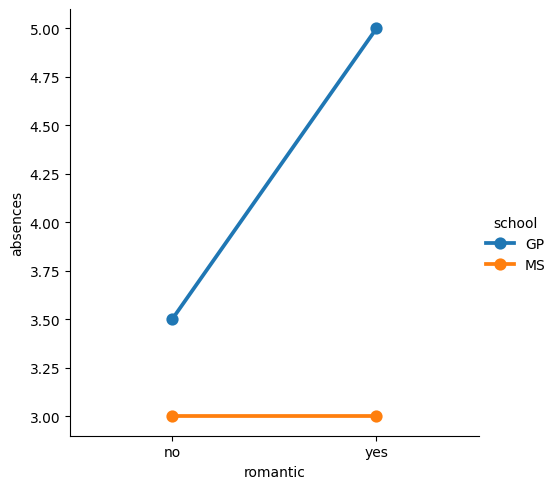
\includegraphics{../images/im295.png}
\end{frame}

\section{Customizing Seaborn Plots}\label{customizing-seaborn-plots}

\begin{frame}{Changing style and palette}
\phantomsection\label{changing-style-and-palette}
Let's return to our dataset containing the results of a survey given to
young people about their habits and preferences.
\end{frame}

\begin{frame}[fragile]{Changing style and palette}
\phantomsection\label{changing-style-and-palette-1}
\AddToHookNext{env/Highlighting/begin}{\tiny}

\begin{Shaded}
\begin{Highlighting}[]
\NormalTok{advice\_mapping }\OperatorTok{=}\NormalTok{ \{}
    \FloatTok{1.0}\NormalTok{: }\StringTok{"Never"}\NormalTok{,}
    \FloatTok{2.0}\NormalTok{: }\StringTok{"Rarely"}\NormalTok{,}
    \FloatTok{3.0}\NormalTok{: }\StringTok{"Sometimes"}\NormalTok{,}
    \FloatTok{4.0}\NormalTok{: }\StringTok{"Often"}\NormalTok{,}
    \FloatTok{5.0}\NormalTok{: }\StringTok{"Always"}\NormalTok{,}
\NormalTok{    np.nan: np.nan  }\CommentTok{\# Keeping NaN as it is}
\NormalTok{\}}
\NormalTok{survey\_data[}\StringTok{"Parents Advice"}\NormalTok{] }\OperatorTok{=}\NormalTok{ survey\_data[}\StringTok{"Parents\textquotesingle{} advice"}\NormalTok{].}\BuiltInTok{map}\NormalTok{(advice\_mapping)}
\end{Highlighting}
\end{Shaded}
\end{frame}

\begin{frame}{Changing style and palette}
\phantomsection\label{changing-style-and-palette-2}
Now let's change the style and palette to make this plot easier to
interpret.
\end{frame}

\begin{frame}{Changing style and palette}
\phantomsection\label{changing-style-and-palette-3}
Set the style to ``whitegrid'' to help the audience determine the number
of responses in each category.
\end{frame}

\begin{frame}[fragile]{Changing style and palette}
\phantomsection\label{changing-style-and-palette-4}
\AddToHookNext{env/Highlighting/begin}{\tiny}

\begin{Shaded}
\begin{Highlighting}[]
\CommentTok{\# Set the style to "whitegrid"}
\NormalTok{sns.set\_style(}\StringTok{"whitegrid"}\NormalTok{)}

\CommentTok{\# Create a count plot of survey responses}
\NormalTok{category\_order }\OperatorTok{=}\NormalTok{ [}\StringTok{"Never"}\NormalTok{, }\StringTok{"Rarely"}\NormalTok{, }\StringTok{"Sometimes"}\NormalTok{, }
                  \StringTok{"Often"}\NormalTok{, }\StringTok{"Always"}\NormalTok{]}

\NormalTok{sns.catplot(x}\OperatorTok{=}\StringTok{"Parents Advice"}\NormalTok{, }
\NormalTok{            data}\OperatorTok{=}\NormalTok{survey\_data, }
\NormalTok{            kind}\OperatorTok{=}\StringTok{"count"}\NormalTok{, }
\NormalTok{            order}\OperatorTok{=}\NormalTok{category\_order)}
\end{Highlighting}
\end{Shaded}
\end{frame}

\begin{frame}{Changing style and palette}
\phantomsection\label{changing-style-and-palette-5}
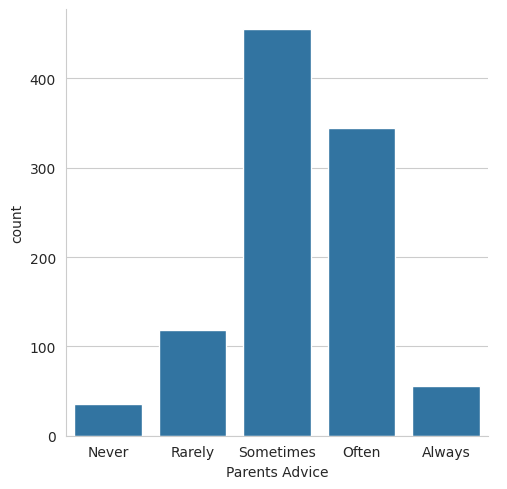
\includegraphics{../images/im296.png}
\end{frame}

\begin{frame}[fragile]{Changing style and palette}
\phantomsection\label{changing-style-and-palette-6}
Set the color palette to the sequential palette named ``Purples''.

\AddToHookNext{env/Highlighting/begin}{\tiny}

\begin{Shaded}
\begin{Highlighting}[]
\CommentTok{\# Set the color palette to "Purples"}
\NormalTok{sns.set\_style(}\StringTok{"whitegrid"}\NormalTok{)}
\NormalTok{sns.set\_palette(}\StringTok{"Purples"}\NormalTok{)}

\CommentTok{\# Create a count plot of survey responses}
\NormalTok{category\_order }\OperatorTok{=}\NormalTok{ [}\StringTok{"Never"}\NormalTok{, }\StringTok{"Rarely"}\NormalTok{, }\StringTok{"Sometimes"}\NormalTok{, }
                  \StringTok{"Often"}\NormalTok{, }\StringTok{"Always"}\NormalTok{]}

\NormalTok{sns.catplot(x}\OperatorTok{=}\StringTok{"Parents Advice"}\NormalTok{, }
\NormalTok{            data}\OperatorTok{=}\NormalTok{survey\_data, }
\NormalTok{            kind}\OperatorTok{=}\StringTok{"count"}\NormalTok{, }
\NormalTok{            order}\OperatorTok{=}\NormalTok{category\_order)}
\end{Highlighting}
\end{Shaded}
\end{frame}

\begin{frame}{Changing style and palette}
\phantomsection\label{changing-style-and-palette-7}
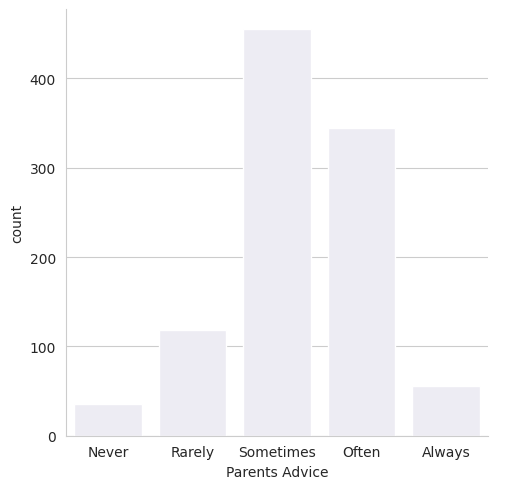
\includegraphics{../images/im297.png}
\end{frame}

\begin{frame}[fragile]{Changing style and palette}
\phantomsection\label{changing-style-and-palette-8}
Change the color palette to the diverging palette named ``RdBu''.

\AddToHookNext{env/Highlighting/begin}{\tiny}

\begin{Shaded}
\begin{Highlighting}[]
\CommentTok{\# Change the color palette to "RdBu"}
\NormalTok{sns.set\_style(}\StringTok{"whitegrid"}\NormalTok{)}
\NormalTok{sns.set\_palette(}\StringTok{"RdBu"}\NormalTok{)}

\CommentTok{\# Create a count plot of survey responses}
\NormalTok{category\_order }\OperatorTok{=}\NormalTok{ [}\StringTok{"Never"}\NormalTok{, }\StringTok{"Rarely"}\NormalTok{, }\StringTok{"Sometimes"}\NormalTok{, }
                  \StringTok{"Often"}\NormalTok{, }\StringTok{"Always"}\NormalTok{]}

\NormalTok{sns.catplot(x}\OperatorTok{=}\StringTok{"Parents Advice"}\NormalTok{, }
\NormalTok{            data}\OperatorTok{=}\NormalTok{survey\_data, }
\NormalTok{            kind}\OperatorTok{=}\StringTok{"count"}\NormalTok{, }
\NormalTok{            order}\OperatorTok{=}\NormalTok{category\_order)}
\end{Highlighting}
\end{Shaded}
\end{frame}

\begin{frame}{Changing style and palette}
\phantomsection\label{changing-style-and-palette-9}
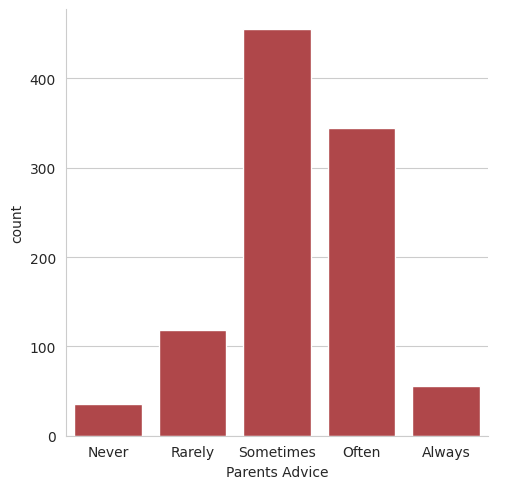
\includegraphics{../images/im298.png}
\end{frame}

\begin{frame}{Changing the scale}
\phantomsection\label{changing-the-scale}
In this exercise, we'll continue to look at the dataset containing
responses from a survey of young people.
\end{frame}

\begin{frame}[fragile]{Changing the scale}
\phantomsection\label{changing-the-scale-1}
\AddToHookNext{env/Highlighting/begin}{\tiny}

\begin{Shaded}
\begin{Highlighting}[]
\ImportTok{import}\NormalTok{ pandas }\ImportTok{as}\NormalTok{ pd}
\ImportTok{import}\NormalTok{ seaborn }\ImportTok{as}\NormalTok{ sns}
\ImportTok{import}\NormalTok{ matplotlib.pyplot }\ImportTok{as}\NormalTok{ plt}

\CommentTok{\# Corrected dataset URL}
\NormalTok{url }\OperatorTok{=} \StringTok{"https://raw.githubusercontent.com/endri81/DataVisualization/main/data/young{-}people{-}survey{-}responses.csv"}

\CommentTok{\# Load the dataset}
\NormalTok{survey\_data }\OperatorTok{=}\NormalTok{ pd.read\_csv(url)}


\CommentTok{\# Define correct column names}
\NormalTok{siblings\_col }\OperatorTok{=} \StringTok{"Siblings"}  \CommentTok{\# Matches dataset}
\NormalTok{lonely\_col }\OperatorTok{=} \StringTok{"Loneliness"}  \CommentTok{\# Corrected from "Feels Lonely"}
\end{Highlighting}
\end{Shaded}
\end{frame}

\begin{frame}[fragile]{Changing the scale}
\phantomsection\label{changing-the-scale-2}
\AddToHookNext{env/Highlighting/begin}{\tiny}

\begin{Shaded}
\begin{Highlighting}[]
\CommentTok{\# Drop missing values in Loneliness}
\NormalTok{survey\_data }\OperatorTok{=}\NormalTok{ survey\_data.dropna(subset}\OperatorTok{=}\NormalTok{[lonely\_col])}

\CommentTok{\# Convert Loneliness to numeric if necessary}
\NormalTok{survey\_data[lonely\_col] }\OperatorTok{=}\NormalTok{ pd.to\_numeric(survey\_data[lonely\_col], errors}\OperatorTok{=}\StringTok{"coerce"}\NormalTok{)}

\CommentTok{\# Convert Siblings to categorical if necessary}
\NormalTok{survey\_data[siblings\_col] }\OperatorTok{=}\NormalTok{ survey\_data[siblings\_col].astype(}\BuiltInTok{str}\NormalTok{)}
\end{Highlighting}
\end{Shaded}
\end{frame}

\begin{frame}{Changing the scale}
\phantomsection\label{changing-the-scale-3}
Does the percentage of people reporting that they feel lonely vary
depending on how many siblings they have?
\end{frame}

\begin{frame}{Changing the scale}
\phantomsection\label{changing-the-scale-4}
Let's find out using a bar plot, while also exploring Seaborn's four
different plot scales (``contexts'').
\end{frame}

\begin{frame}{Changing the scale}
\phantomsection\label{changing-the-scale-5}
Set the scale (``context'') to ``paper'', which is the smallest of the
scale options.
\end{frame}

\begin{frame}[fragile]{Changing the scale}
\phantomsection\label{changing-the-scale-6}
\AddToHookNext{env/Highlighting/begin}{\tiny}

\begin{Shaded}
\begin{Highlighting}[]
\CommentTok{\# Set seaborn context}
\NormalTok{sns.set\_context(}\StringTok{"paper"}\NormalTok{)}

\CommentTok{\# Create bar plot using the correct column name}
\NormalTok{sns.catplot(x}\OperatorTok{=}\NormalTok{siblings\_col, y}\OperatorTok{=}\NormalTok{lonely\_col, }
\NormalTok{            data}\OperatorTok{=}\NormalTok{survey\_data, kind}\OperatorTok{=}\StringTok{"bar"}\NormalTok{, errorbar}\OperatorTok{=}\VariableTok{None}\NormalTok{)}

\CommentTok{\# Show the plot}
\NormalTok{plt.show()}
\end{Highlighting}
\end{Shaded}
\end{frame}

\begin{frame}{Changing the scale}
\phantomsection\label{changing-the-scale-7}
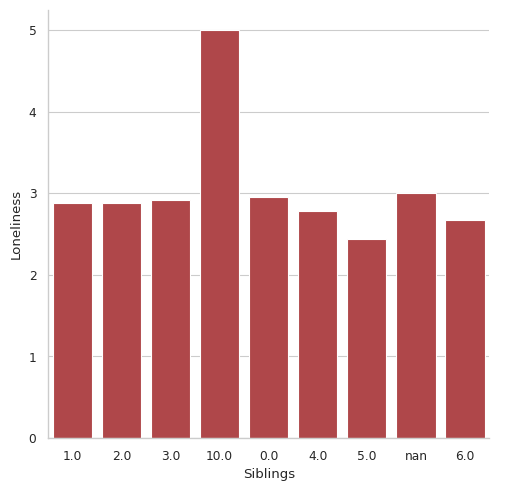
\includegraphics{../images/im299.png}
\end{frame}

\begin{frame}{Changing the scale}
\phantomsection\label{changing-the-scale-8}
Change the context to ``notebook'' to increase the scale.
\end{frame}

\begin{frame}[fragile]{Changing the scale}
\phantomsection\label{changing-the-scale-9}
\AddToHookNext{env/Highlighting/begin}{\tiny}

\begin{Shaded}
\begin{Highlighting}[]
\CommentTok{\# Set seaborn context}
\NormalTok{sns.set\_context(}\StringTok{"notebook"}\NormalTok{)}

\CommentTok{\# Create bar plot using the correct column name}
\NormalTok{sns.catplot(x}\OperatorTok{=}\NormalTok{siblings\_col, y}\OperatorTok{=}\NormalTok{lonely\_col, }
\NormalTok{            data}\OperatorTok{=}\NormalTok{survey\_data, kind}\OperatorTok{=}\StringTok{"bar"}\NormalTok{, errorbar}\OperatorTok{=}\VariableTok{None}\NormalTok{)}

\CommentTok{\# Show the plot}
\NormalTok{plt.show()}
\end{Highlighting}
\end{Shaded}
\end{frame}

\begin{frame}{Changing the scale}
\phantomsection\label{changing-the-scale-10}
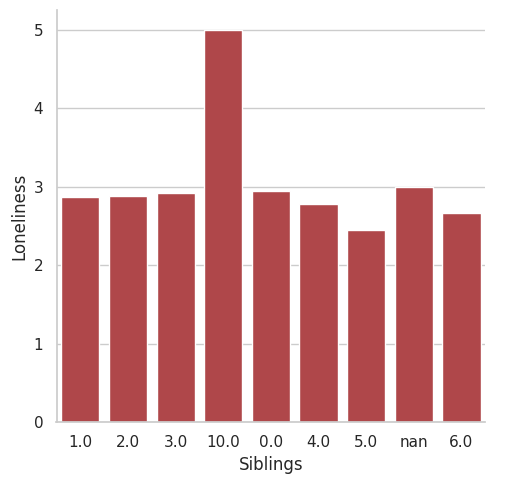
\includegraphics{../images/im300.png}
\end{frame}

\begin{frame}{Changing the scale}
\phantomsection\label{changing-the-scale-11}
Change the context to ``talk'' to increase the scale.
\end{frame}

\begin{frame}[fragile]{Changing the scale}
\phantomsection\label{changing-the-scale-12}
\AddToHookNext{env/Highlighting/begin}{\tiny}

\begin{Shaded}
\begin{Highlighting}[]
\CommentTok{\# Set seaborn context}
\NormalTok{sns.set\_context(}\StringTok{"talk"}\NormalTok{)}

\CommentTok{\# Create bar plot using the correct column name}
\NormalTok{sns.catplot(x}\OperatorTok{=}\NormalTok{siblings\_col, y}\OperatorTok{=}\NormalTok{lonely\_col, }
\NormalTok{            data}\OperatorTok{=}\NormalTok{survey\_data, kind}\OperatorTok{=}\StringTok{"bar"}\NormalTok{, errorbar}\OperatorTok{=}\VariableTok{None}\NormalTok{)}

\CommentTok{\# Show the plot}
\NormalTok{plt.show()}
\end{Highlighting}
\end{Shaded}
\end{frame}

\begin{frame}{Changing the scale}
\phantomsection\label{changing-the-scale-13}
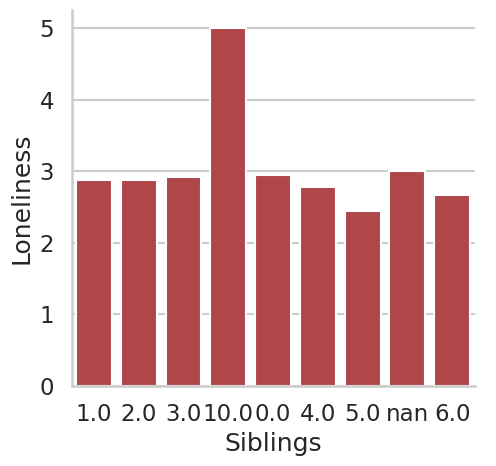
\includegraphics{../images/im301.png}
\end{frame}

\begin{frame}{Changing the scale}
\phantomsection\label{changing-the-scale-14}
Change the context to ``poster'', which is the largest scale available.
\end{frame}

\begin{frame}[fragile]{Changing the scale}
\phantomsection\label{changing-the-scale-15}
\AddToHookNext{env/Highlighting/begin}{\tiny}

\begin{Shaded}
\begin{Highlighting}[]
\CommentTok{\# Set seaborn context}
\NormalTok{sns.set\_context(}\StringTok{"poster"}\NormalTok{)}

\CommentTok{\# Create bar plot using the correct column name}
\NormalTok{sns.catplot(x}\OperatorTok{=}\NormalTok{siblings\_col, y}\OperatorTok{=}\NormalTok{lonely\_col, }
\NormalTok{            data}\OperatorTok{=}\NormalTok{survey\_data, kind}\OperatorTok{=}\StringTok{"bar"}\NormalTok{, errorbar}\OperatorTok{=}\VariableTok{None}\NormalTok{)}

\CommentTok{\# Show the plot}
\NormalTok{plt.show()}
\end{Highlighting}
\end{Shaded}
\end{frame}

\begin{frame}{Changing the scale}
\phantomsection\label{changing-the-scale-16}
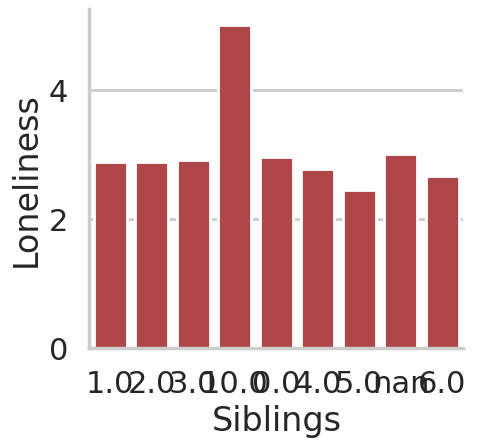
\includegraphics{../images/im302.png}
\end{frame}

\begin{frame}{Using a custom palette}
\phantomsection\label{using-a-custom-palette}
So far, we've looked at several things in the dataset of survey
responses from young people, including their internet usage, how often
they listen to their parents, and how many of them report feeling
lonely.
\end{frame}

\begin{frame}{Using a custom palette}
\phantomsection\label{using-a-custom-palette-1}
However, one thing we haven't done is a basic summary of the type of
people answering this survey, including their age and gender.

Providing these basic summaries is always a good practice when dealing
with an unfamiliar dataset.
\end{frame}

\begin{frame}{Using a custom palette}
\phantomsection\label{using-a-custom-palette-2}
The code provided will create a box plot showing the distribution of
ages for male versus female respondents. Let's adjust the code to
customize the appearance, this time using a custom color palette.
\end{frame}

\begin{frame}{Using a custom palette}
\phantomsection\label{using-a-custom-palette-3}
Set the style to ``darkgrid''.

Set a custom color palette with the hex color codes ``\#39A7D0'' and
``\#36ADA4''.
\end{frame}

\begin{frame}[fragile]{Using a custom palette}
\phantomsection\label{using-a-custom-palette-4}
\AddToHookNext{env/Highlighting/begin}{\tiny}

\begin{Shaded}
\begin{Highlighting}[]
\CommentTok{\# Set the style to "darkgrid"}
\NormalTok{sns.set\_style(}\StringTok{"darkgrid"}\NormalTok{)}

\CommentTok{\# Set a custom color palette}
\NormalTok{sns.set\_palette([}\StringTok{"\#39A7D0"}\NormalTok{, }\StringTok{"\#36ADA4"}\NormalTok{])}

\CommentTok{\# Create the box plot of age distribution by gender}
\NormalTok{sns.catplot(x}\OperatorTok{=}\StringTok{"Gender"}\NormalTok{, y}\OperatorTok{=}\StringTok{"Age"}\NormalTok{, }
\NormalTok{            data}\OperatorTok{=}\NormalTok{survey\_data, kind}\OperatorTok{=}\StringTok{"box"}\NormalTok{)}
\end{Highlighting}
\end{Shaded}
\end{frame}

\begin{frame}{Using a custom palette}
\phantomsection\label{using-a-custom-palette-5}
\includegraphics{../images/im303.png}
\end{frame}

\begin{frame}{FacetGrids vs.~AxesSubplots}
\phantomsection\label{facetgrids-vs.-axessubplots}
In the recent lesson, we learned that Seaborn plot functions create two
different types of objects: FacetGrid objects and AxesSubplot objects.
\end{frame}

\begin{frame}{FacetGrids vs.~AxesSubplots}
\phantomsection\label{facetgrids-vs.-axessubplots-1}
The method for adding a title to your plot will differ depending on the
type of object it is.
\end{frame}

\begin{frame}{FacetGrids vs.~AxesSubplots}
\phantomsection\label{facetgrids-vs.-axessubplots-2}
In the code provided, we've used relplot() with the miles per gallon
dataset to create a scatter plot showing the relationship between a
car's weight and its horsepower.

This scatter plot is assigned to the variable name g. Let's identify
which type of object it is.
\end{frame}

\begin{frame}[fragile]{FacetGrids vs.~AxesSubplots}
\phantomsection\label{facetgrids-vs.-axessubplots-3}
\AddToHookNext{env/Highlighting/begin}{\tiny}

\begin{Shaded}
\begin{Highlighting}[]
\CommentTok{\# Create scatter plot}
\NormalTok{g }\OperatorTok{=}\NormalTok{ sns.relplot(x}\OperatorTok{=}\StringTok{"weight"}\NormalTok{, }
\NormalTok{                y}\OperatorTok{=}\StringTok{"horsepower"}\NormalTok{, }
\NormalTok{                data}\OperatorTok{=}\NormalTok{mpg,}
\NormalTok{                kind}\OperatorTok{=}\StringTok{"scatter"}\NormalTok{)}

\CommentTok{\# Identify plot type}
\NormalTok{type\_of\_g }\OperatorTok{=} \BuiltInTok{type}\NormalTok{(g)}

\CommentTok{\# Print type}
\NormalTok{plt.close()  }\CommentTok{\# added/edited}
\BuiltInTok{print}\NormalTok{(type\_of\_g)}
\end{Highlighting}
\end{Shaded}
\end{frame}

\begin{frame}{FacetGrids vs.~AxesSubplots}
\phantomsection\label{facetgrids-vs.-axessubplots-4}
\includegraphics{../images/im304.png}
\end{frame}

\begin{frame}{Adding a title to a FacetGrid object}
\phantomsection\label{adding-a-title-to-a-facetgrid-object}
In the previous exercise, we used relplot() with the miles per gallon
dataset to create a scatter plot showing the relationship between a
car's weight and its horsepower.

This created a FacetGrid object. Now that we know what type of object it
is, let's add a title to this plot.
\end{frame}

\begin{frame}{Adding a title to a FacetGrid object}
\phantomsection\label{adding-a-title-to-a-facetgrid-object-1}
Add the following title to this plot: ``Car Weight vs.~Horsepower''.
\end{frame}

\begin{frame}[fragile]{Adding a title to a FacetGrid object}
\phantomsection\label{adding-a-title-to-a-facetgrid-object-2}
\AddToHookNext{env/Highlighting/begin}{\tiny}

\begin{Shaded}
\begin{Highlighting}[]
\CommentTok{\# Create scatter plot}
\NormalTok{g }\OperatorTok{=}\NormalTok{ sns.relplot(x}\OperatorTok{=}\StringTok{"weight"}\NormalTok{, }
\NormalTok{                y}\OperatorTok{=}\StringTok{"horsepower"}\NormalTok{, }
\NormalTok{                data}\OperatorTok{=}\NormalTok{mpg,}
\NormalTok{                kind}\OperatorTok{=}\StringTok{"scatter"}\NormalTok{)}

\CommentTok{\# Add a title "Car Weight vs. Horsepower"}
\NormalTok{g.fig.suptitle(}\StringTok{"Car Weight vs. Horsepower"}\NormalTok{)}

\CommentTok{\# Show plot}
\NormalTok{plt.show()}
\end{Highlighting}
\end{Shaded}
\end{frame}

\begin{frame}{Adding a title to a FacetGrid object}
\phantomsection\label{adding-a-title-to-a-facetgrid-object-3}
\includegraphics{../images/im305.png}
\end{frame}

\begin{frame}{Adding a title and axis labels}
\phantomsection\label{adding-a-title-and-axis-labels}
Let's continue to look at the miles per gallon dataset.

This time we'll create a line plot to answer the question:
\end{frame}

\begin{frame}{Adding a title and axis labels}
\phantomsection\label{adding-a-title-and-axis-labels-1}
How does the average miles per gallon achieved by cars change over time
for each of the three places of origin?

To improve the readability of this plot, we'll add a title and more
informative axis labels.
\end{frame}

\begin{frame}{Adding a title and axis labels}
\phantomsection\label{adding-a-title-and-axis-labels-2}
In the code provided, we create the line plot using the lineplot()
function.

Note that lineplot() does not support the creation of subplots, so it
returns an AxesSubplot object instead of an FacetGrid object.
\end{frame}

\begin{frame}[fragile]{Adding a title and axis labels}
\phantomsection\label{adding-a-title-and-axis-labels-3}
\AddToHookNext{env/Highlighting/begin}{\tiny}

\begin{Shaded}
\begin{Highlighting}[]
\NormalTok{mpg\_mean }\OperatorTok{=}\NormalTok{ mpg.groupby([}\StringTok{"model\_year"}\NormalTok{, }\StringTok{"origin"}\NormalTok{]).agg(mpg\_mean}\OperatorTok{=}\NormalTok{(}\StringTok{"mpg"}\NormalTok{, }\StringTok{"mean"}\NormalTok{)).reset\_index()}
\CommentTok{\# Create line plot}
\NormalTok{g }\OperatorTok{=}\NormalTok{ sns.lineplot(x}\OperatorTok{=}\StringTok{"model\_year"}\NormalTok{, y}\OperatorTok{=}\StringTok{"mpg\_mean"}\NormalTok{, }
\NormalTok{                 data}\OperatorTok{=}\NormalTok{mpg\_mean,}
\NormalTok{                 hue}\OperatorTok{=}\StringTok{"origin"}\NormalTok{)}

\CommentTok{\# Add a title "Average MPG Over Time"}
\NormalTok{g.set\_title(}\StringTok{"Average MPG Over Time"}\NormalTok{)}

\CommentTok{\# Show plot}
\NormalTok{plt.show()}
\end{Highlighting}
\end{Shaded}
\end{frame}

\begin{frame}{Adding a title and axis labels}
\phantomsection\label{adding-a-title-and-axis-labels-4}
\includegraphics{../images/im306.png}
\end{frame}

\begin{frame}[fragile]{Adding a title and axis labels}
\phantomsection\label{adding-a-title-and-axis-labels-5}
\AddToHookNext{env/Highlighting/begin}{\tiny}

\begin{Shaded}
\begin{Highlighting}[]
\CommentTok{\# Create line plot}
\NormalTok{g }\OperatorTok{=}\NormalTok{ sns.lineplot(x}\OperatorTok{=}\StringTok{"model\_year"}\NormalTok{, y}\OperatorTok{=}\StringTok{"mpg\_mean"}\NormalTok{, }
\NormalTok{                 data}\OperatorTok{=}\NormalTok{mpg\_mean,}
\NormalTok{                 hue}\OperatorTok{=}\StringTok{"origin"}\NormalTok{)}

\CommentTok{\# Add a title "Average MPG Over Time"}
\NormalTok{g.set\_title(}\StringTok{"Average MPG Over Time"}\NormalTok{)}

\CommentTok{\# Add x{-}axis and y{-}axis labels}
\NormalTok{g.}\BuiltInTok{set}\NormalTok{(xlabel}\OperatorTok{=}\StringTok{"Car Model Year"}\NormalTok{, }
\NormalTok{      ylabel}\OperatorTok{=}\StringTok{"Average MPG"}\NormalTok{)}

\CommentTok{\# Show plot}
\NormalTok{plt.show()}
\end{Highlighting}
\end{Shaded}
\end{frame}

\begin{frame}{Adding a title and axis labels}
\phantomsection\label{adding-a-title-and-axis-labels-6}
\includegraphics{../images/im307.png}
\end{frame}

\begin{frame}{Rotating x-tick labels}
\phantomsection\label{rotating-x-tick-labels}
In this exercise, we'll continue looking at the miles per gallon
dataset.

In the code provided, we create a point plot that displays the average
acceleration for cars in each of the three places of origin.
\end{frame}

\begin{frame}{Rotating x-tick labels}
\phantomsection\label{rotating-x-tick-labels-1}
Note that the ``acceleration'' variable is the time to accelerate from 0
to 60 miles per hour, in seconds. Higher values indicate slower
acceleration.

Let's use this plot to practice rotating the x-tick labels.
\end{frame}

\begin{frame}{Rotating x-tick labels}
\phantomsection\label{rotating-x-tick-labels-2}
Recall that the function to rotate x-tick labels is a standalone
Matplotlib function and not a function applied to the plot object
itself.
\end{frame}

\begin{frame}[fragile]{Rotating x-tick labels}
\phantomsection\label{rotating-x-tick-labels-3}
Rotate the x-tick labels 90 degrees.

\AddToHookNext{env/Highlighting/begin}{\tiny}

\begin{Shaded}
\begin{Highlighting}[]

\CommentTok{\# Create point plot}
\NormalTok{sns.catplot(x}\OperatorTok{=}\StringTok{"origin"}\NormalTok{, }
\NormalTok{            y}\OperatorTok{=}\StringTok{"acceleration"}\NormalTok{, }
\NormalTok{            data}\OperatorTok{=}\NormalTok{mpg, }
\NormalTok{            kind}\OperatorTok{=}\StringTok{"point"}\NormalTok{, }
\NormalTok{            join}\OperatorTok{=}\VariableTok{False}\NormalTok{, }
\NormalTok{            capsize}\OperatorTok{=}\FloatTok{0.1}\NormalTok{)}
\end{Highlighting}
\end{Shaded}
\end{frame}

\begin{frame}[fragile]{Rotating x-tick labels}
\phantomsection\label{rotating-x-tick-labels-4}
\AddToHookNext{env/Highlighting/begin}{\tiny}

\begin{Shaded}
\begin{Highlighting}[]
\CommentTok{\# Rotate x{-}tick labels}
\NormalTok{plt.xticks(rotation}\OperatorTok{=}\DecValTok{90}\NormalTok{)}
\CommentTok{\#\# ([0, 1, 2], [Text(0, 0, \textquotesingle{}usa\textquotesingle{}), Text(1, 0, \textquotesingle{}japan\textquotesingle{}), Text(2, 0, \textquotesingle{}europe\textquotesingle{})])}
\CommentTok{\# Show plot}
\NormalTok{plt.show()}
\end{Highlighting}
\end{Shaded}
\end{frame}

\begin{frame}{Rotating x-tick labels}
\phantomsection\label{rotating-x-tick-labels-5}
\includegraphics{../images/im308.png}
\end{frame}

\begin{frame}{Box plot with subgroups}
\phantomsection\label{box-plot-with-subgroups}
In this exercise, we'll look at the dataset containing responses from a
survey given to young people.

One of the questions asked of the young people was: ``Are you interested
in having pets?''
\end{frame}

\begin{frame}{Box plot with subgroups}
\phantomsection\label{box-plot-with-subgroups-1}
Let's explore whether the distribution of ages of those answering
``yes'' tends to be higher or lower than those answering ``no'',
controlling for gender.
\end{frame}

\begin{frame}{Box plot with subgroups}
\phantomsection\label{box-plot-with-subgroups-2}
Set the color palette to ``Blues''.
\end{frame}

\begin{frame}[fragile]{Box plot with subgroups}
\phantomsection\label{box-plot-with-subgroups-3}
\AddToHookNext{env/Highlighting/begin}{\tiny}

\begin{Shaded}
\begin{Highlighting}[]
\NormalTok{survey\_data }\OperatorTok{=}\NormalTok{ pd.read\_csv(}\StringTok{"survey\_data.csv"}\NormalTok{)}
\CommentTok{\# Set palette to "Blues"}
\NormalTok{sns.set\_palette(}\StringTok{"Blues"}\NormalTok{)}
\end{Highlighting}
\end{Shaded}
\end{frame}

\begin{frame}{Box plot with subgroups}
\phantomsection\label{box-plot-with-subgroups-4}
Add subgroups to color the box plots based on ``Interested in Pets''.
\end{frame}

\begin{frame}[fragile]{Box plot with subgroups}
\phantomsection\label{box-plot-with-subgroups-5}
\AddToHookNext{env/Highlighting/begin}{\tiny}

\begin{Shaded}
\begin{Highlighting}[]
\CommentTok{\# Adjust to add subgroups based on "Interested in Pets"}
\NormalTok{g }\OperatorTok{=}\NormalTok{ sns.catplot(x}\OperatorTok{=}\StringTok{"Gender"}\NormalTok{,}
\NormalTok{                y}\OperatorTok{=}\StringTok{"Age"}\NormalTok{, data}\OperatorTok{=}\NormalTok{survey\_data, }
\NormalTok{                kind}\OperatorTok{=}\StringTok{"box"}\NormalTok{, hue}\OperatorTok{=}\StringTok{"Pets"}\NormalTok{)}
\end{Highlighting}
\end{Shaded}
\end{frame}

\begin{frame}{Box plot with subgroups}
\phantomsection\label{box-plot-with-subgroups-6}
\includegraphics{../images/im309.png}
\end{frame}

\begin{frame}{Box plot with subgroups}
\phantomsection\label{box-plot-with-subgroups-7}
Set the title of the FacetGrid object g to ``Age of Those Interested in
Pets vs.~Not''.
\end{frame}

\begin{frame}[fragile]{Box plot with subgroups}
\phantomsection\label{box-plot-with-subgroups-8}
\AddToHookNext{env/Highlighting/begin}{\tiny}

\begin{Shaded}
\begin{Highlighting}[]
\CommentTok{\# Set title to "Age of Those Interested in Pets vs. Not"}
\NormalTok{g.fig.suptitle(}\StringTok{"Age of Those Interested in Pets vs. Not"}\NormalTok{)}

\CommentTok{\# Show plot}
\NormalTok{plt.show()}
\end{Highlighting}
\end{Shaded}
\end{frame}

\begin{frame}{Box plot with subgroups}
\phantomsection\label{box-plot-with-subgroups-9}
\includegraphics{../images/im310.png}
\end{frame}

\begin{frame}{Bar plot with subgroups and subplots}
\phantomsection\label{bar-plot-with-subgroups-and-subplots}
In this exercise, we'll return to our young people survey dataset and
investigate whether the proportion of people who like techno music
(``Likes Techno'') varies by their gender (``Gender'') or where they
live (``Village - town'').
\end{frame}

\begin{frame}{Bar plot with subgroups and subplots}
\phantomsection\label{bar-plot-with-subgroups-and-subplots-1}
This exercise will give us an opportunity to practice the many things
we've learned throughout this course!
\end{frame}

\begin{frame}{Bar plot with subgroups and subplots}
\phantomsection\label{bar-plot-with-subgroups-and-subplots-2}
Set the figure style to ``dark''.

Adjust the bar plot code to add subplots based on ``Gender'', arranged
in columns.

Add the title ``Percentage of Young People Who Like Techno'' to this
FacetGrid plot.

Label the x-axis ``Location of Residence'' and y-axis ``\% Who Like
Techno''.
\end{frame}

\begin{frame}[fragile]{Bar plot with subgroups and subplots}
\phantomsection\label{bar-plot-with-subgroups-and-subplots-3}
\AddToHookNext{env/Highlighting/begin}{\tiny}

\begin{Shaded}
\begin{Highlighting}[]
\CommentTok{\# Set the figure style to "dark"}
\NormalTok{sns.set\_style(}\StringTok{"dark"}\NormalTok{)}

\CommentTok{\# Adjust to add subplots per gender}
\NormalTok{g }\OperatorTok{=}\NormalTok{ sns.catplot(x}\OperatorTok{=}\StringTok{"Village {-} town"}\NormalTok{, y}\OperatorTok{=}\StringTok{"Likes Techno"}\NormalTok{, }
\NormalTok{                data}\OperatorTok{=}\NormalTok{survey\_data, kind}\OperatorTok{=}\StringTok{"bar"}\NormalTok{,}
\NormalTok{                col}\OperatorTok{=}\StringTok{"Gender"}\NormalTok{)}

\CommentTok{\# Add title and axis labels}
\NormalTok{g.fig.suptitle(}\StringTok{"Percentage of Young People Who Like Techno"}\NormalTok{, y}\OperatorTok{=}\FloatTok{1.02}\NormalTok{)}
\NormalTok{g.}\BuiltInTok{set}\NormalTok{(xlabel}\OperatorTok{=}\StringTok{"Location of Residence"}\NormalTok{, }
\NormalTok{      ylabel}\OperatorTok{=}\StringTok{"\% Who Like Techno"}\NormalTok{)}
\end{Highlighting}
\end{Shaded}
\end{frame}

\begin{frame}{Box plot with subgroups}
\phantomsection\label{box-plot-with-subgroups-10}
\includegraphics{../images/im311.png}
\end{frame}

\end{document}
